\chapter{User-Guided Mesh Simplification}
\label{topstoc0}

\begin{flushright}
\textit{``The original motivation to do research [that led to technological discoveries]\\was to expand the range of possibilities for storytellers.''}\\
-- Ed Catmull {[}at the 73rd Scientific and Technical Academy Awards, 2001{]}
\end{flushright}

In this section we finally want to connect the theoretical part with the practical application.
We will illustrate the workings our reference implementation\footnote{ Our reference implementation was written in STL conform \texttt{C++}. The only dependancies are \href{http://www.openmesh.org/}{OpenMesh} which provides the data structure for the mesh operations, \href{http://www.qtcentre.org/content/}{Qt} for the \texttt{GUI} and \href{http://www.libqglviewer.com/}{libQGLViewer} that facilitates the incorporation of \texttt{OpenGL} for the view-port. Although the core algorithms are very lean, the entire code-basis has grown to well over 4000 lines of code over the course of the thesis.
Right now, most parts are not appropriately documented, but after some annotations are added, it will be made available -- fell free to inquire via \href{mailto:mail@lnpe.at}{mail@lnpe.at}.} and discuss our results.\\
First, we will briefly describe the so called ``TopStoc'' algorithm in section \ref{topstoc1}.
It serves as the core decimation method to which the other tools were added.
The following three subsections \ref{topstoc121}, \ref{topstoc122} and \ref{topstoc123}, discuss three useful adaptations of ``TopStoc'' that we made use of.

The next section \ref{topstoc2} then lays out the topological aspects.
\ref{topstoc21} details the tools for getting accurate and useful information like the genus, Betti numbers and of course the handle and tunnel loops as well as open boundaries, which are also subsumed as topological important loops.
This information about the mesh serves in as much as it helps the user deciding which characteristics he wants to alter.  
Besides the tools to change the topology, described in \ref{topstoc22}, we will also talk about the limitations of our approach in \ref{topstoc23}.

The rest of the chapter from section \ref{topstoc3} to \ref{topstoc43} then illustrates further ways of valuable user-interaction and how to leverage guidance as well as practical considerations like support for textures \ref{topstoc42}.
Last but not least, we will come to talk about how to measure and evaluate results of any decimation and the two principe paradigms \ref{topstoc51} and \ref{topstoc52} we found most suitable to work with.


\section{The TopStoc Algorithm}
\label{topstoc1}

The basis for our work are the two algorithms described in the paper ``Stochastic Sampling and Topological Clustering'' \citep[cf.][]{Boubekeur2009}.
The main advantage over other solutions, undoubtedly is its speed, typically surpassing the quasi decimation standard ``QSlim'' by an order of magnitude.
Consequently it is a natural fit for any system that wants to offer smooth interaction for user-guidance. 
%Bild
\begin{figure}[ht]
\centering
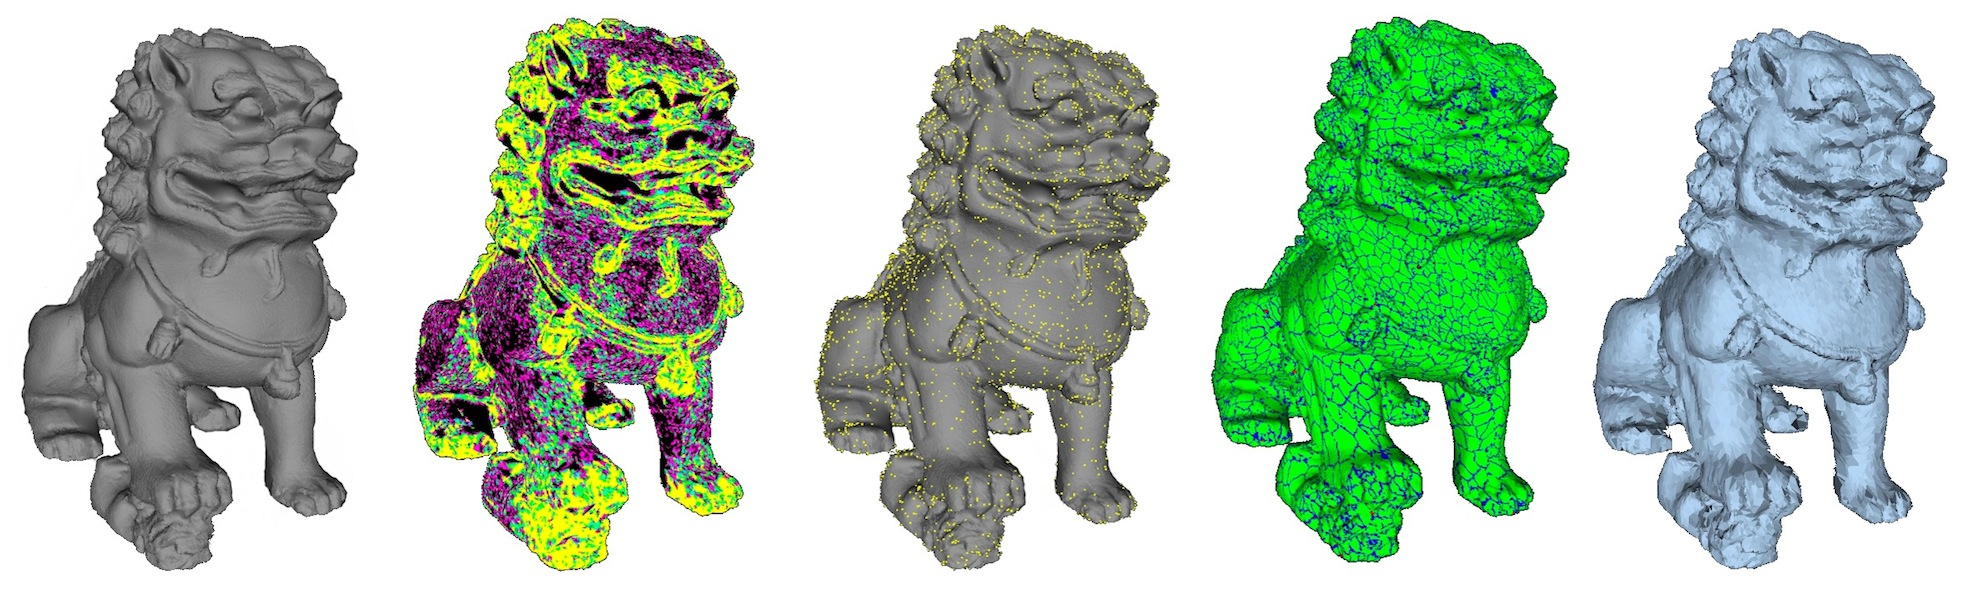
\includegraphics[width=1.0\textwidth]{topstoc_dragons.jpg}
\caption{Results from our TopStoc implementation, left to right: The base mesh; visualization of the local normal deviation; sampled vertices that define the low-resolution mesh; visualization of the topological clustering; the final mesh.}
\label{fig:topstoc_dragons}
\end{figure}\\
Before we can treat any modifications we give an ``as short as possible'' rundown of the individual steps, as laid out in the original paper:
%\vspace{-2ex}
\begin{itemize}
%\setlength{\itemsep}{0cm} \setlength{\parskip}{0cm}
	\item \textit{Stochastic Vertex Selection} -- to select the ``best'' vertices for a low resolution model, every vertex is assigned a value $\mathrm{x}$ of geometric importance, we refer to as weight: \begin{equation} \label{eq:vertex_weight}
\mathrm{x}(\mathrm{v}) \,=\, \frac{|\mathrm{N}_{v}| - \sum_{\mathrm{u} \in \mathrm{N}_{v} } (\textbf{n}^{T}_{v}\textbf{n}_{u})}{2 \cdot |\mathrm{N}_{v}|}
\end{equation}
In other words, for every vertex the normal deviation of its immediate surroundings, i.e. the so called one-ring of vertex normals is calculated. Depending on the weight of each vertex and the target size, a subsample is selected. Note that the probability distribution must be tweaked, so that subsampling in flat areas is avoided. The second and third dragon in figure \ref{fig:topstoc_dragons} show the vertex weight respectively a sampling.
	\item \textit{Topological Clustering} -- the sampled vertices are used to partition the mesh via a breadth-first flood-filling. This way ever vertex of the base mesh is allotted to one representative. Following the idea of vertex clustering each of the sub-meshes is used to retriangulate the surface, but instead of spatial distance the topological proximity defines a grid cell, so to say. Thus contrary to normal clustering the homotopy of base and decimated mesh is ensured. The penultimate dragon in figure \ref{fig:topstoc_dragons} shows the result of the flood-filling. Green areas mark a topological cells, blue triangles the boarder between any two of them and red face indicates an intersection of three different cells that determine the connectivity of the new mesh.
	\item \textit{Density Control} -- not part of the basic decimation suit, is this method a way to improve the shapes of the resulting triangles. Obviously there are already many other concepts to refine triangles, but most of them are very costly. Density control avoids this relapse to high complexity by using a strategy inspired by ``Poisson disk'' rejection sampling. Just before the sampled vertices are used in the topological cluster stage, each neighborhood of a sampled vertex removes any other sampling within a given distance threshold. 
\end{itemize}


\subsection{Fast Topological Clustering}
\label{topstoc121}

As already mentioned, both the stochastic vertex selection as well as the topological clustering are both very fast.
However, of these two, the latter is considerably slower than the first.
Not only is the clustering more algorithmically complex, but also is there no immediate way to quickly accelerate it.
The calculation of weights and the selection of vertices can be trivially sped up by implementing a parallelized version of the algorithm, as every individual decision is completely independent of the other calculations\footnote{ Given that every SIMD threat has access, not only to one vertex, but also the adjacent vertices.}.
For this reason we are more interested in improving the clustering stage and propose a small modification that particularly pays of for cases in which the target sizes is small, i.e. below 10\%.

The algorithm in its original version only needs the set of sampled vertices $\overline{\mathcal{V}}$ and a queue $\mathrm{Q}$ to store vertex references, besides means to navigate the neighborhood of any vertex on the surface of course.
During the flood-fill every vertex of the base mesh gets touched at least once to assign the mark of the cell it belongs to, see algorithm \ref{algo:topological_clustering}.
Only to then iterate once more over the entire mesh to check whether three different cell marks coincide on a given face.
%Algorithm
\begin{table}[htb] \medskip \centering
\setlength{\tabcolsep}{5pt}
\renewcommand{\arraystretch}{1.10}
\fbox{
	\begin{minipage}{10cm}
	\begin{tabular}{r | l} 
				&	\textsc{Breadth-first flood-filling ($\overline{\mathcal{V}}$)} \\[1ex]
		\tiny{1}	&	\hspace{0.2cm}	\textsf{for each vertex $\mathrm{v}$ in $\overline{\mathcal{V}}$ do} \\
		\tiny{2}	&	\hspace{1.0cm}	\textsf{mark $\mathrm{v}$ with $\mathrm{v}$} \\
		\tiny{3}	&	\hspace{1.0cm}	\textsf{append reference of $\mathrm{v}$ to $\mathrm{Q}$} \\
		\tiny{4}	&	\hspace{0.2cm}	\textsf{end for} \\
		\tiny{5}	&	\hspace{0.2cm}	\textsf{while $\mathrm{Q}$ is not empty do} \\
		\tiny{6}	&	\hspace{1.0cm}	\textsf{$\mathrm{v} :=$ head of $\mathrm{Q}$} \\
		\tiny{7}	&	\hspace{1.0cm}	\textsf{for each vertex $\mathrm{u}$ in $\mathrm{N}_{V}[\mathrm{v}]$ do} \\
		\tiny{8}	&	\hspace{1.6cm}	\textsf{if $\mathrm{u}$ is not marked then} \\		
		\tiny{9}	&	\hspace{2.0cm}	\textsf{mark $\mathrm{u}$ with mark of $\mathrm{v}$} \\
		\tiny{10}	&	\hspace{2.0cm}	\textsf{append $\mathrm{u}$ to $\mathrm{Q}$} \\
		\tiny{+11}&	\hspace{1.6cm}	\textsf{else if mark is different to $\mathrm{v}$ then} \\
		\tiny{+12}&	\hspace{2.0cm}	\textsf{append the associated face $\mathrm{f}_{\mathrm{u}}$ to $\mathrm{L}$} \\
		\tiny{13}	&	\hspace{1.6cm}	\textsf{end if} \\
		\tiny{14}	&	\hspace{1.0cm}	\textsf{end for} \\
		\tiny{15}	&	\hspace{1.0cm}	\textsf{pop head of $\mathrm{Q}$} \\
		\tiny{16}	&	\hspace{0.2cm}	\textsf{end while} \\[1ex]
	\end{tabular} \end{minipage}
}
	\medskip
	\caption{Algorithm -- Breadth-first flood-filling.}
	\label{algo:topological_clustering}
\end{table}\\
In the modified version we, include one more \textsf{else if} condition at the time when a vertex would be normally passed on for the reason that it is already marked.
We check whether the mark of vertex $\mathrm{v}$, with which another vertex $\mathrm{u}$ should have been marked are identical.
In the case that vertex $\mathrm{u}$ can't be marked by $\mathrm{v}$ because it was previously marked, there are two scenarios.
Either it was already marked by $\mathrm{v}$ during an earlier step of the flood-fill, or it was marked by a different vertex $\mathrm{s}$.
Note that in the end, what we are ultimately interested in, is finding only the faces where all three vertices were marked by separate vertices.
Hence, if vertex $\mathrm{v}$ encounters an already marked vertex $\mathrm{u}$ that bears the same mark as itself, it is impossible for the two adjacent faces of the edge connecting $\mathrm{v}$ and $\mathrm{u}$ to be one of these interesting faces.\\
Understanding this, we append faces to an unique list $\mathrm{L}$, i.e. without allowing multiple entries, if during the flood-fill two different marks where found.
The new steps in the algorithm are marked with '$+$' in \ref{algo:topological_clustering}.
Note that we only add one face $\mathrm{f}_{u}$ to $\mathrm{L}$, not both, this is because the check will happen two times from both sides starting with either vertex once.
In order to skip the second face and avoid unnecessary multiple insertions, we have to be consistent, attaching either the face of the outgoing or the incoming half-edge only.

%Bild
\begin{figure}[hbt]
\centering
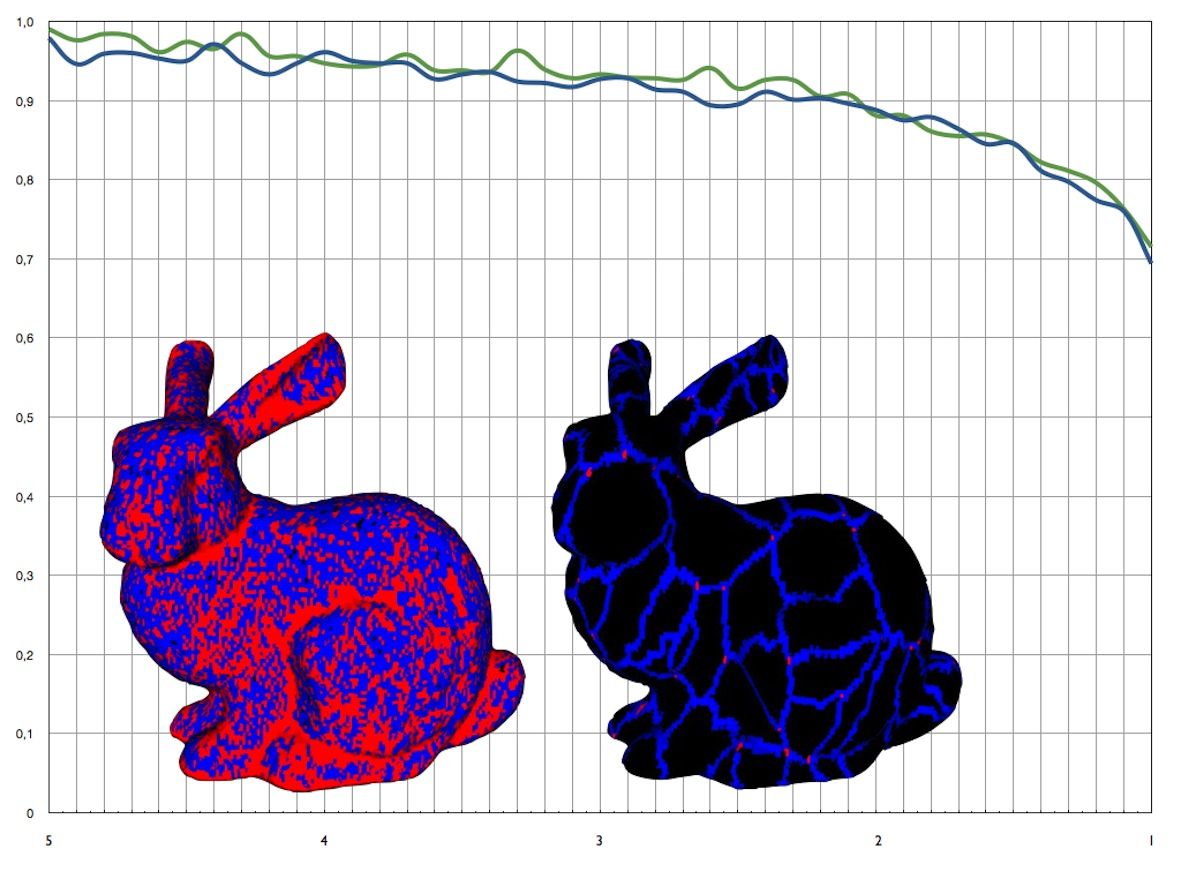
\includegraphics[width=1.0\textwidth]{fast_clustering.jpg}
\caption{The Y-axsis shows the relative improvement in \% of the list size of faces to check (blue and yellow) and the runtime (red and green) for decimation ratios between 0.5 and 0.01 on the X-axis. The two bunnies demonstrate the results for a very high and a very low sampling, omitted faces are visualized in black.}
\label{fig:fast_clustering}
\end{figure}
Although the final list of faces to check holds far less references, runtime improvements manifest themselves only for high decimation rates.
This is due to the fact that inserting faces to the list $\mathrm{L}$ is costly.\\
For example for decimation of the \textit{Chinese Dragon} Model, from initially over 655,000 vertices to about 5\%, the runtime decreased about 15\%.
For target sizes around 1\% the speed-ups can be far greater, at about 30\%.
In figure \ref{fig:fast_clustering} we plotted the size reduction of the List $\mathrm{L}$ for two models, namely the \textit{Stanford Bunny} and the \textit{Chinese Dragon} -- indicated by the blue and orange curve, as well as the relative runtime to the unmodified version shown by the curves in red and green\footnote{ Each measurement was taken multiple times in 1\% steps for the interval of 50\% down to 1\%. $\frac{\mathcal{F}}{\mathrm{L}$} blue (\textit{Stanford Bunny}) and yellow (\textit{Chinese Dragon}) and $\frac{t_{fast}}{t_{normal}}$ -- green (\textit{Stanford Bunny}) and red (\textit{Chinese Dragon}). }.\\
As the target size is known before the flood-fill occurs, we automatically use this feature in case the the target size is smaller than 50\%\,\footnote{ Note that ``TopStoc'' in general is better suited for high decimation ratios, as its advantages over other solutions are diminished at low decimation rates >50\%.}.

\newpage
\subsection{Adaptive Density Control}
\label{topstoc122}

Density control as introduced in the original paper can greatly improve the quality of decimated mesh triangulation.
Having said that, it has suffers two drawbacks. 
One is the fact that the mesh resembles more and more what one would expect form a uniform sampling as the distance $\epsilon$, in which samples are removed, increases. 
Thereby negating the intention and design of the the stochastic selection phase of the vertices.
The second problem is that the clean-up process can increase the runtime noticeably, up to 50\%.
%Bild
\begin{figure}[ht]
\centering
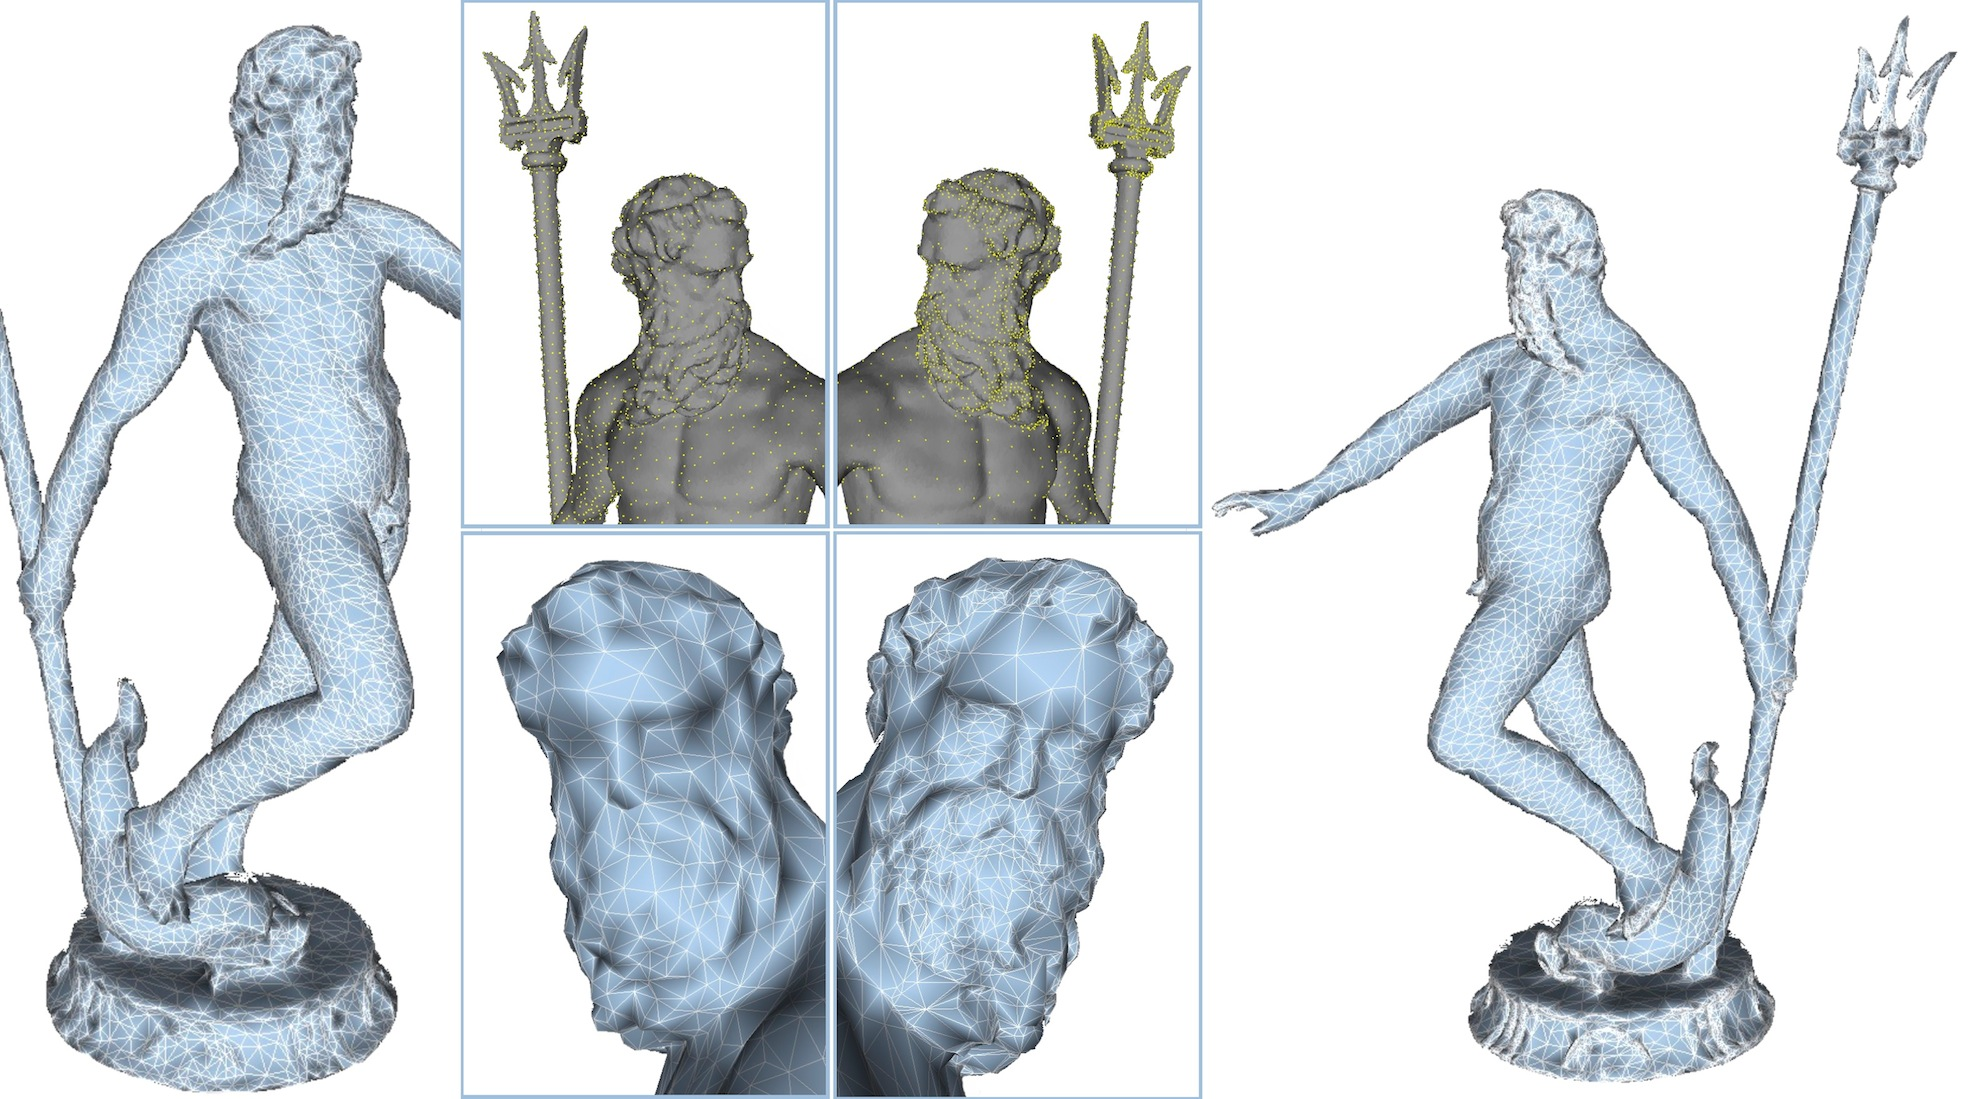
\includegraphics[width=1.0\textwidth]{adaptive_density_control.jpg}
\caption{Normal vs. adaptive density control. Whereas the sampling left shows almost uniform distribution, the adaptive version retains higher vertex counts in important regions without loosing good aspect ratios of the triangles. Note how the triangle size changes between forehead and beard.}
\label{fig:adaptive_density_control}
\end{figure}\\
We propose two simple modifications to mitigate these effects, which we call \textit{Adaptive Density Control}.
Ideally we want good triangle shapes without loosing too much geometric detail.
To solve this problem we simply vary the cleansing distance $\epsilon_{v}$ according to the weight of the vertex $\mathrm{v}$ it is associated with.
In shows the results for the \textit{Neptune} Model \ref{fig:adaptive_density_control}.
On the left one can see the decimated mesh after isotropic or normal density control was used.
For the results on the right model we adapted the distance $\epsilon$ to just two values.
$\epsilon_{big}$ if the vertex weight was below the mean vertex weight: $\mathrm{x}(\mathrm{v}) < \overline{\mathrm{x}}$ and to $\epsilon_{small}$ if the vertex weight was above the mean vertex weight: $\mathrm{x}(\mathrm{v}) > \overline{\mathrm{x}}$, with $\epsilon_{small} < \epsilon_{big}$.
Note that the value $\overline{\mathrm{x}}$ gets calculated during the sampling phase and is already given at that point.

We did not specify exact values in our example, neither for $\epsilon_{big}$, nor for $\epsilon_{small}$.
The reason for this is, that instead of euclidian distances as originally proposed, we opted for measuring the distances in terms of so called 1-rings instead\footnote{ This concept depends to some extend on the assumption that edge lengths will not drastically vary in local neighborhoods. We think this is a sound assumptions, for some applications like marching cubes or Delaunay generated surfaces this holds by definition. However should the user see that a given surfaces is not suitable the euclidean distance measure with an continuous $\epsilon \in [\mathrm{d}_{min}, \mathrm{d}_{max}]$ can always be used as a fall-back alternative.}.
This means for instance, that every sampled vertex with a weight $\mathrm{x}(\mathrm{v}) > \overline{\mathrm{x}}$ only evaluates its direct neighboring vertices $\epsilon_{small} = 1$, whereas a vertex with $\mathrm{x}(\mathrm{v}) < \overline{\mathrm{x}}$ will spread out much like the cells during flood-fill, we achieved good results for $\frac{\epsilon_{big}}{\epsilon_{small}} \geq 2$.
%Bild
\begin{figure}[ht]
\centering
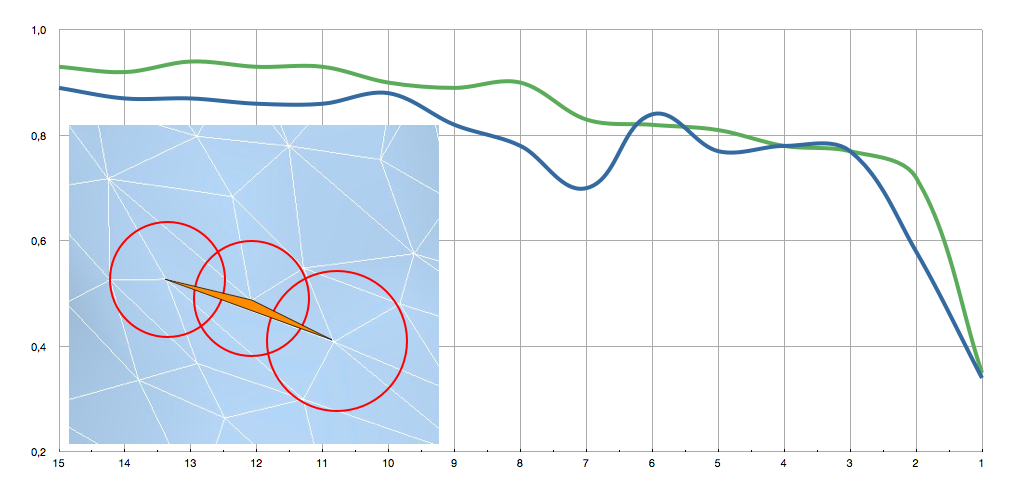
\includegraphics[width=1.0\textwidth]{bad_triangles.jpg}
\caption{Relative triangle quality, Y-axis, of normal decimation (blue) vs. density control (green), over small decimation ratios X-axis and an example of a bad triangle shape that can't be caught by density control.}
\label{fig:bad_triangles}
\end{figure}\\
Not having to calculate euclidian distances greatly improves the runtime, unfortunately one problem still retains that hasn't been mentioned at all, so far.
While tinkering with adaptive density control, we calculated the aspect ratios of the triangles to have quantitative benchmarks.
The aspect ratio of a triangle $\mathrm{f}$ is a dimensionless number $AR \in [1, \infty)$, that is 1 if and only if for all edges $||\mathrm{e}_{i}|| = ||\mathrm{e}_{j}||$:
\begin{equation} \label{eq:aspect_ratio}
\mathrm{AR}(\mathrm{f}) \,=\, \frac{||\mathrm{e}_{0}|| \cdot ||\mathrm{e}_{1}|| \cdot ||\mathrm{e}_{2}||}{8 \cdot (s-||\mathrm{e}_{0}||) \cdot (s-||\mathrm{e}_{1}||) \cdot (s-||\mathrm{e}_{2}||)}, ~~~~ s = \frac{||\mathrm{e}_{0}|| + ||\mathrm{e}_{1}|| + ||\mathrm{e}_{2}||}{2}
\end{equation}
After looking at the data we notices the the ratio between the mean and maximum value for all faces: $AR(\mathcal{M}) := \frac{AR_{mean}}{AR_{max}}$ did not turn out as expected.
First and most importantly, they weren't as good as hoped.
Drilling down on the issue showed that only $AR_{mean}$ improved and that $AR_{max}$ still remained high.
This is especially worrisome as for example, simulations are not resilient against single bad triangles no matter how good the rest are.
The second finding was that the ratio $AR(\mathcal{M})$ is highly volatile and can vary greatly from sample to sample.\\
In figure \ref{fig:bad_triangles} we plotted $AR(\mathcal{M})$ on the Y-axis, over the target size of the decimation, X-axis.
The blue curve is the result for decimations without any density control, and green shows the results with normal density control.
Although generally better, judging only by the diagram, density control hardly merits its expenses.
Yet, optically the results are convincing.
The conundrum can be explained with the example from the triangulation in \ref{fig:bad_triangles}.
All three vertices of the badly shaped, orange, triangle have a big surrounding that was cleared by the density control step, but still this does not guarantee good shapes, as they nevertheless can be poorly arranged.\\
In order to circumvent this problem one can run a conventional clean-up step at the very end, which also means that the runtime drastically increases.
Up to this point we do not have a viable solution that securely rids every single bad triangles from the mesh without breaking time complexity of the otherwise fast density control.


\subsection{Saving Sample Data}
\label{topstoc123}

By no means a big addition, but a helpful supplement, is the option to save the references of sampled vertices.
Since the topological clustering will result the exact version of a decimated mesh, as long as the order of the vertex queue $\mathrm{Q}$ is preserved and the underlying mesh does not change.\\
This enables the user to save any specific decimation at almost no memory cost.
So instead of saving the entire meshes for various discrete LODs, the user can carefully edit each version, including any manual tweaks like setting control points, etc. and save only the short and efficient list of references.
Once the geometry of a mesh is loaded and only a different version is needed, this strategy can lead to huge difference in loading times, especially when dealing with big models.


\newpage
\section{Simplifying Topology}
\label{topstoc2}

\subsection{Information \& Feature Detection}
\label{topstoc21}

Our goal is to provide the user with clear and unambiguous information, so that he can easily decide whether to dismiss or keep a topological feature.
It took the entire chapter \ref{math0}, to lay down the mathematical foundations and to introduce the algorithms needed, especially the pairing of simplices \ref{algo:simplex_pairing}.
Now we want to show the results.
%Bild
\begin{figure}[ht]
\centering
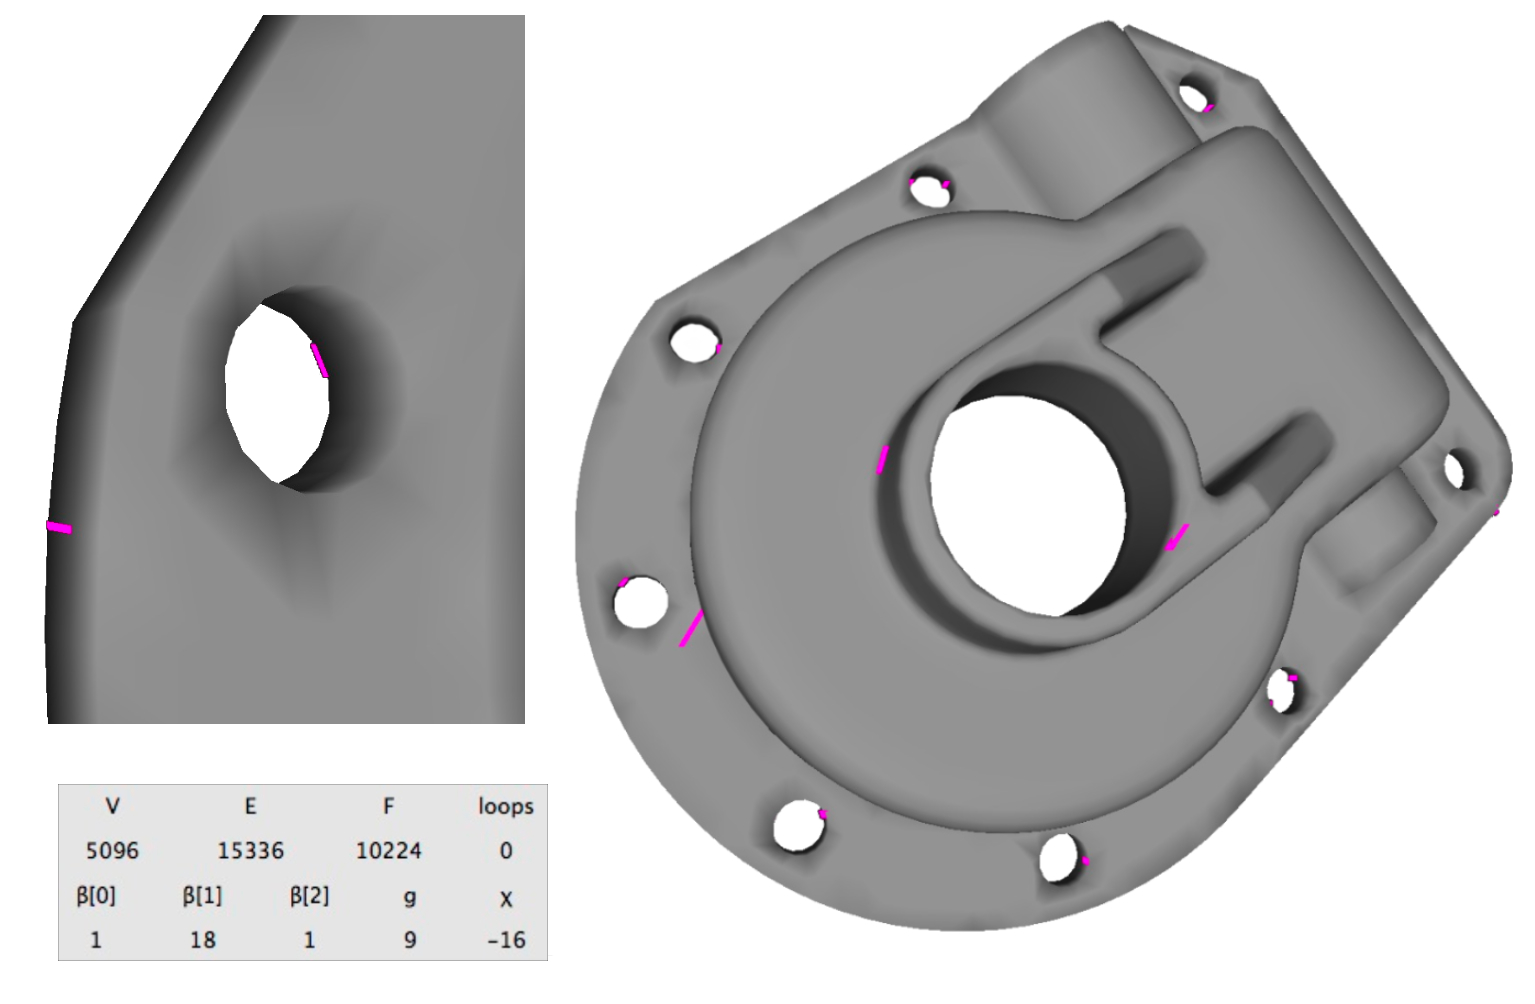
\includegraphics[width=0.85\textwidth]{casting.jpg}
\caption{The model \textit{Casting}, of genus 9 with the handle and tunnel loops inducing edges visualized.}
\label{fig:casting}
\end{figure}\\
At any time the user is presented with a control panel displaying the following topological relevant information:
%\vspace{-2ex}
\begin{itemize}
%\setlength{\itemsep}{0cm} \setlength{\parskip}{0cm}
	\item \textit{V, E, F} -- the total number of vertices, edges and faces, i.e. the number of simplices.
	\item \textit{$\beta$[0] / $\beta$[1] / $\beta$[2]} -- the Betti numbers, which are determined once all simplices of the surface mesh have been paired. As soon as the filtration has finished, the unpaired edges that define handles and tunnel can be visualized too. In figure \ref{fig:casting} the mesh is of genus 9, producing 18 edges, which are colored pink.\\The exact location of these edges depends on the filtration, however we generally observed that they mostly stick very closely to ``their'' features. The further an unpaired edge is away, the more likely it is to get paired by a positive face face of low persistence as a positive face will pair with the first negative edge it encounters during the expansion of its boundary $\partial \Prefix^{+}{\sigma^{2}}$.
	\item \textit{g \& $\chi$} -- the genus respectively the Euler–Poincaré characteristic. If a boundary edge, i.e. an edge only adjacent to one face, is encountered while the mesh is loaded, the exact number of boundaries gets determined. This is necessary in order to calculate the genus: $\chi = 2-2g-boundaries$. Note that this does not apply if the mesh is already filtered, as the Betti numbers are accurate regardless whether the simplicial complex $\mathrm{K}$ is closed or not, see also equation \ref{eq:euler_poincare}.
	\item \textit{loops} -- shows either the number of open boundary loops or the sum of the handle and tunnel loops. The latter can only be detected after once the mesh is closed, as their definition relies on the distinction between the inside $\mathrm{K}_{\mathbb{I}$ and outside volume $\mathrm{K}_{\mathbb{O}$ of the mesh, see subsection \ref{math_loop_computation}.  
\end{itemize}
%Bild
\begin{figure}[ht]
\centering
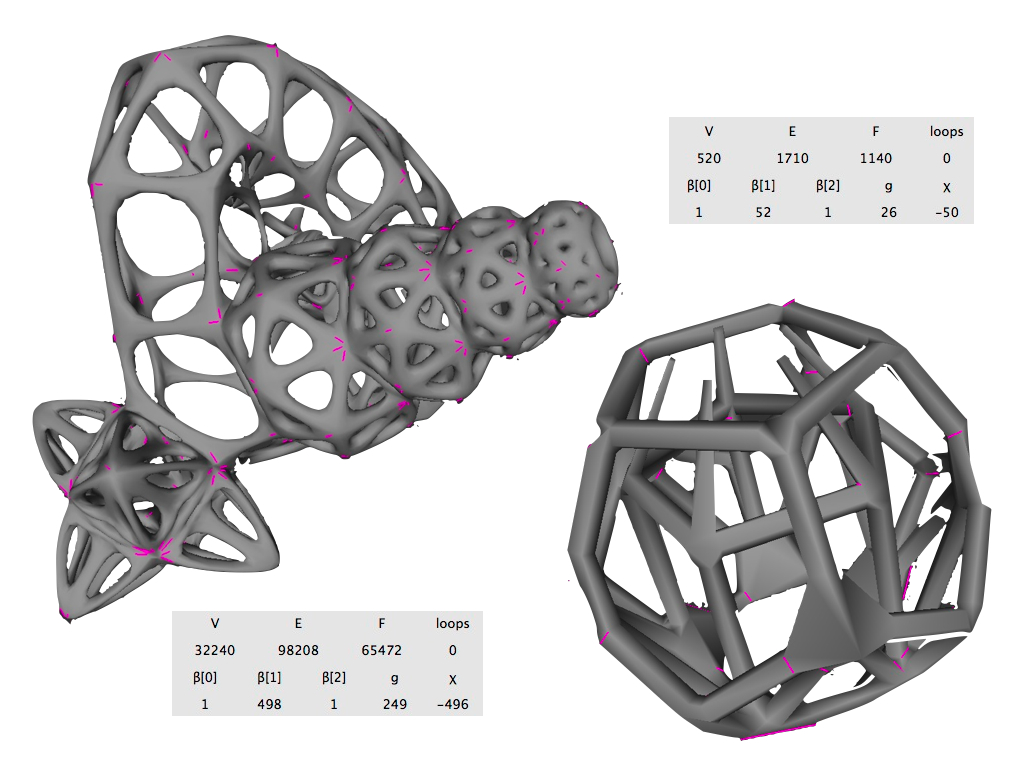
\includegraphics[width=0.80\textwidth]{high_genus.jpg}
\caption{Two ornamental models with high genera and their unpaired edges colored.}
\label{fig:high_genus}
\end{figure}\\
Note that the complexity of the pairing algorithm does not depend on the genus, only on the total number of simplices $|\sigma^{n}|$ with $n>0$, that constitute $\mathrm{K}$.
It is further noteworthy that the time needed to pair all simplices of a dimension $n>m$ gets exponentially bigger as not only the size of the boundary $\partial_{n} > \partial_{m}$ also increase and with it the number of chain elements that get introduced during every step of the expansion.

The decision if a particular unpaired edge gives rise to a handle or a tunnel can only be made after the simplices of the inside, respectively outside have been added to the filtration.
%Bild
\begin{figure}[ht]
\centering
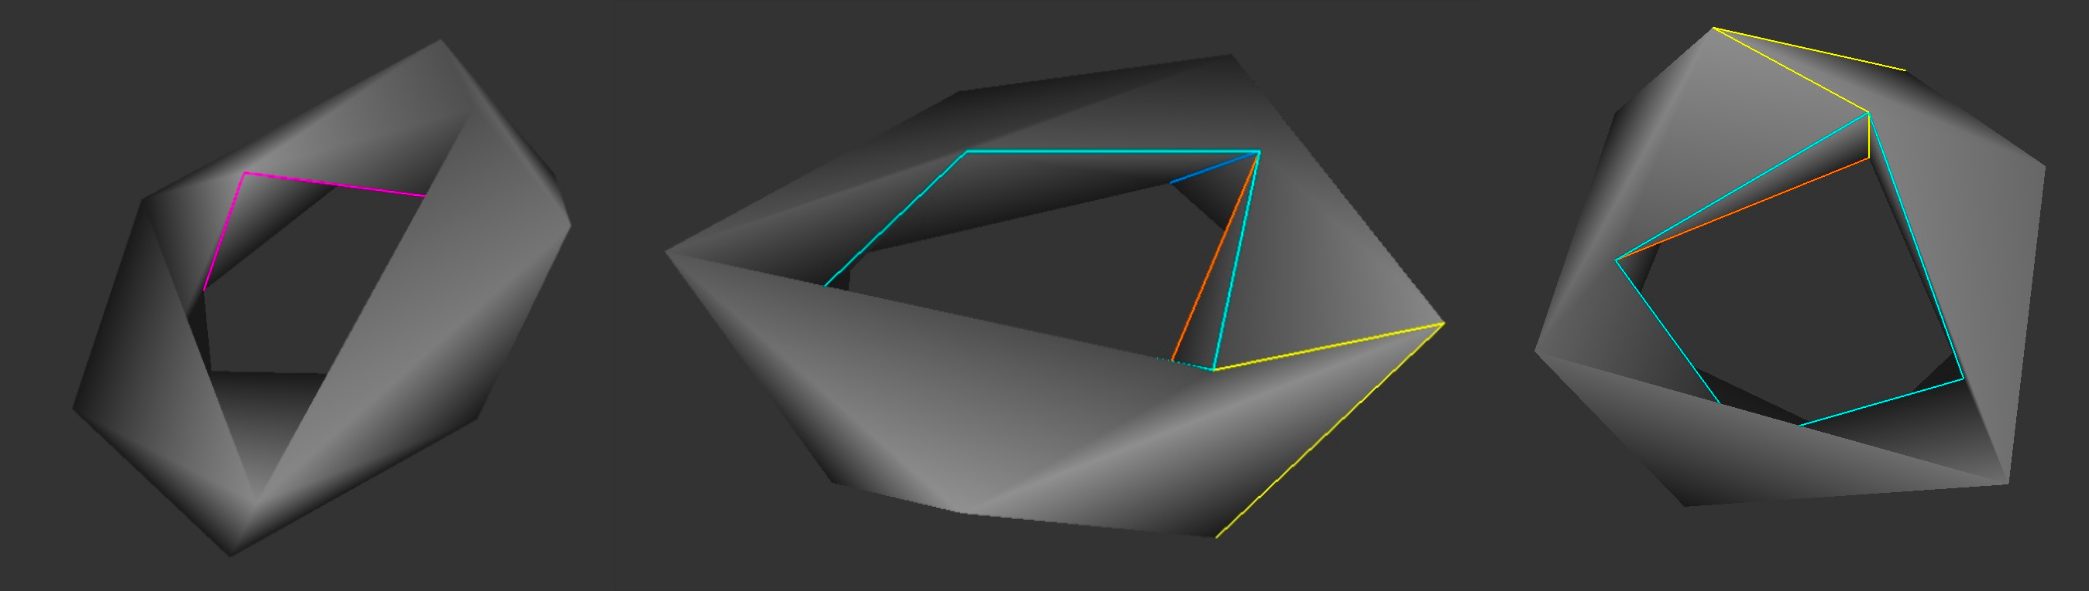
\includegraphics[width=1.0\textwidth]{found_loops.jpg}
\caption{A tunnel (turquoise) and handle (yellow) loop of a simple torus with its paired edges in blue and orange.}
\label{fig:found_loops}
\end{figure}\\
In figure \ref{fig:found_loops} the two unpaired edges of the torus are pink until it is clear which edge belongs to the tunnel loop, here colored in turquoise, and which belongs to the handle loop, colored yellow.
The formerly undifferentiated edges now get colored \textit{tunnel $\rightarrow$ blue} and \textit{handle $\rightarrow$ orange} to show their dependancies\footnote{ Much to our grievance, at the time of penning this thesis, we still have a problem with the \texttt{TetGen} library that we envisioned to use for the tetrahedralization of the surface mesh. Because of this we can only present handle and tunnel loops for the simple tori as its tetrahedralization was done and checked manually.\\Regardless of this unfavorable situation it could be argued that this step could be skipped altogether. This sounds like an extreme measure and motivated by the problems we encountered using particular external libraries. But it is a valid point, as the number of total simplices increases at about ca. 5x because of a tetrahedralization and with it the complexity of the pairing algorithm. In light of this immense computational cost it becomes questionable to go the extra mile, just in order to get a few connected edges. One can make the point that since the unpaired edges are enough to indicate topological features, the user has enough information to decide if he wants to alter the topology or not. One possible direction to pursuit is to filter the surface mesh, thus ensuring with absolute certainty that all important features get represented, but then switching to a cheap heuristic that orders the edges by importance by using some local estimator.}.


\subsection{Mesh Editing}
\label{topstoc22}

Independent from feature detection, the user always has the option to manually select any face of the mesh and delete it.
Besides the deletion tool, the users second instrument to change topology is the retriangulate of an boundary loop.\\
In figure \ref{fig:cut_and_mend} this is shown exemplarily for a double torus that gets dissected by hand in two places.
The deletion on the left kills a handle loop and the deletion on the right kills a tunnel loop.
After the cuts, the mesh gets filtered again to update the Betti numbers -- note that $\chi$ remains -2, this is not an error, it is correct for the reason that we introduced 4 new boundaries.
To indicate the boundaries, the vertices on them are colored red.
As long as the mesh has open boundaries, the user can cycle through them via buttons and retriangulate them\footnote{ Retriangulating holes in surface meshes, is by no means a trivial task and many papers have been published, devoted to answering this question \citep[cf.][]{Zhao2007}. Yet, we assume that any hole filling happens at places of minor importance, typically to mend the mesh after an unimportant feature has been deleted. Additionally we don't care for the quality as long as it produces a water-tight sealing. Consequently we do not deploy a sophisticated scheme but instead project the boundary onto a plane and use a 2D triangulation algorithm to solve the problem.}.
The currently selected boundary is shown via the color yellow.\\
%Bild
\begin{figure}[ht]
\centering
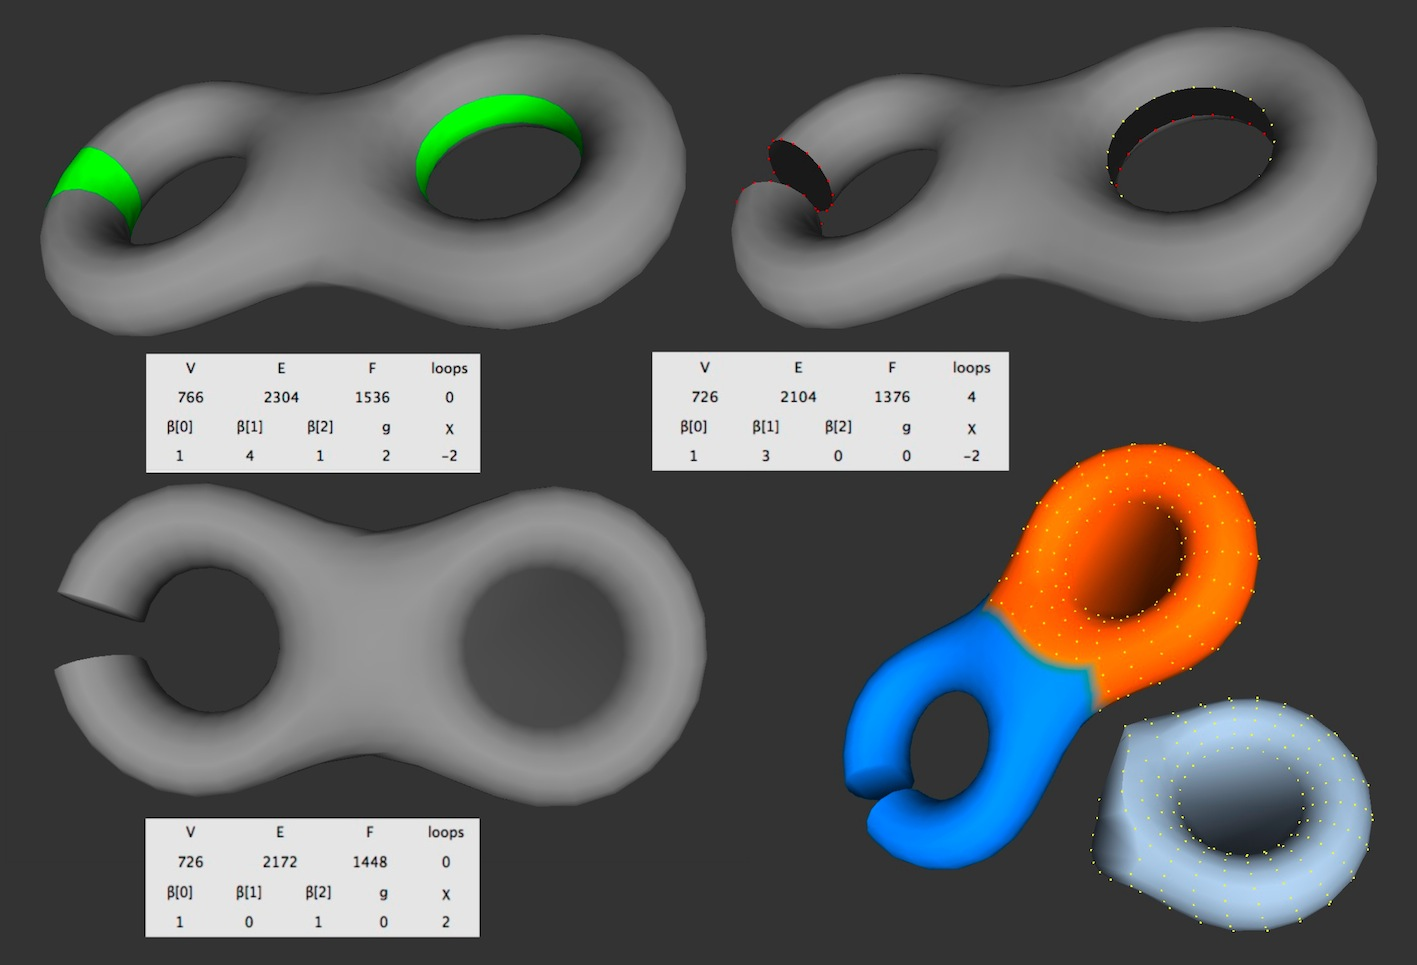
\includegraphics[width=1.0\textwidth]{cut_and_mend.jpg}
\caption{Topological operatons on a double torus.}
\label{fig:cut_and_mend}
\end{figure}\\
After the four boundaries are retriangulated the mesh is topologically equivalent to a sphere as indicated by the invariants.
To further prove the successful transformation we set the sampling probability for half of the mesh to zero -- blue region, and to one for the other half -- orange region.
On the lower right of figure \ref{fig:cut_and_mend} is the outcome, a decimated mesh with genus null.

\newpage
\subsection{Limitations}
\label{topstoc23}

There are two limitations to consider when working with the current implementation.
The first being that our implementation was designed to work with one single connected component at a time.
If a mesh should get partitioned into two individuals parts, the program has no way to display the topological invariants individually.
Interestingly enough though, the algorithm does still work and reckoning the change is trivial as $\beta^{0}>1$, see figure \ref{fig:g3_cut}.
Note that the although the Betti numbers are correct the reported genus for the second mesh is plain wrong.
At this point, reconnecting parts that were split before, is not supported. 
%Bild
\begin{figure}[ht]
\centering
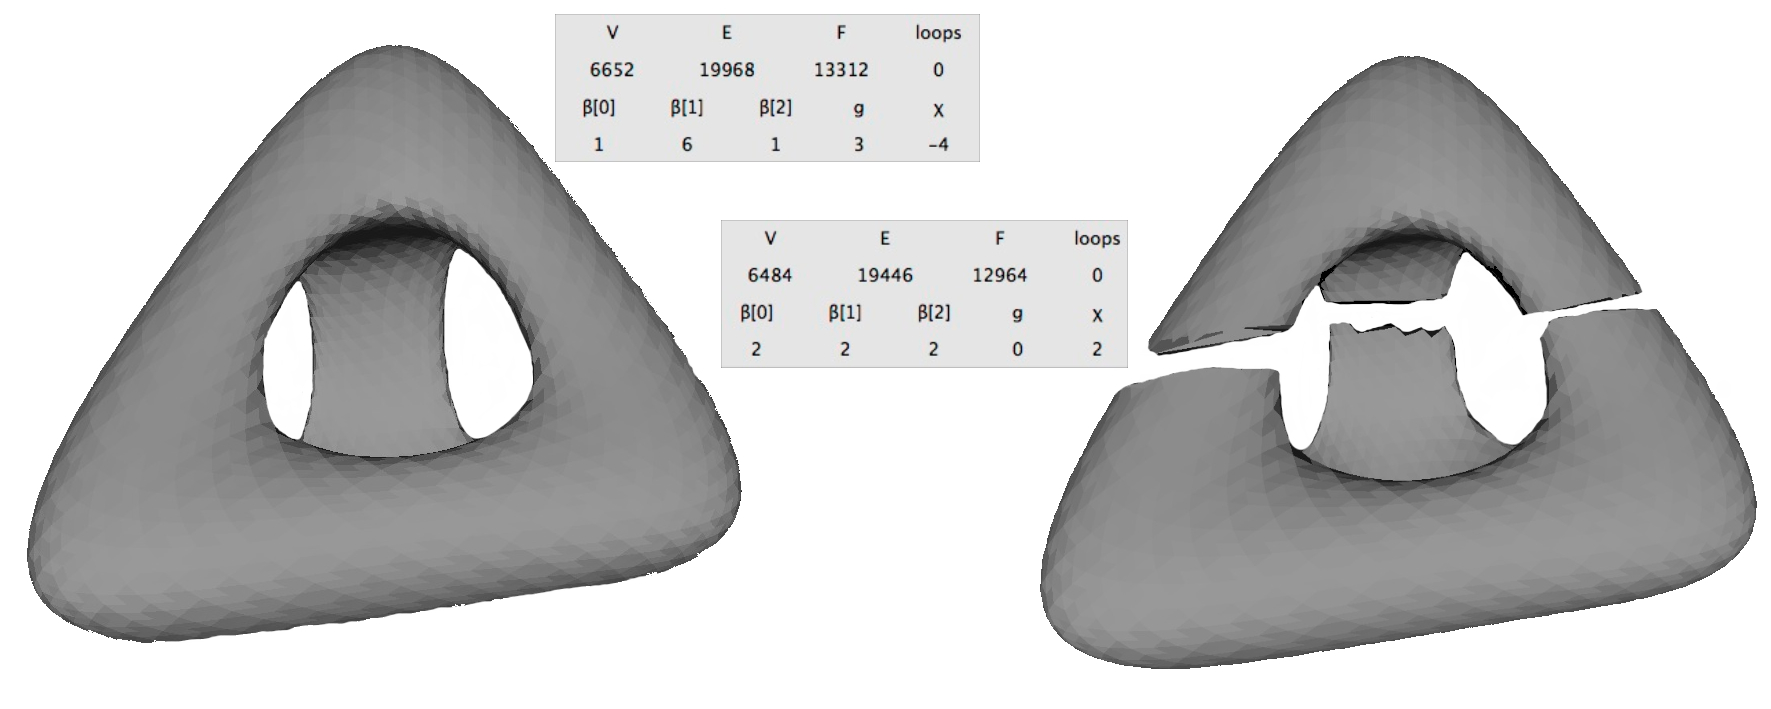
\includegraphics[width=0.75\textwidth]{g3_cut.jpg}
\caption{A mesh $g=3$ that gets severed into two parts, with $g_{1}=0$ and $g_{2}=1$ .}
\label{fig:g3_cut}
\end{figure}\\
The second restrictions concerns not orientable surfaces.
This is more of a barrier, as the pairing algorithm completely fails and even displays boundary vertices for the completely closed mesh.
Even our viewport fails in the face of this challenge, when asked to render triangles, as seen on the right sight of figure \ref{fig:klein_bottle}.
For that matter, the TopStoc algorithm can't be convinced to work with this type of meshes either.
%Bild
\begin{figure}[ht]
\centering
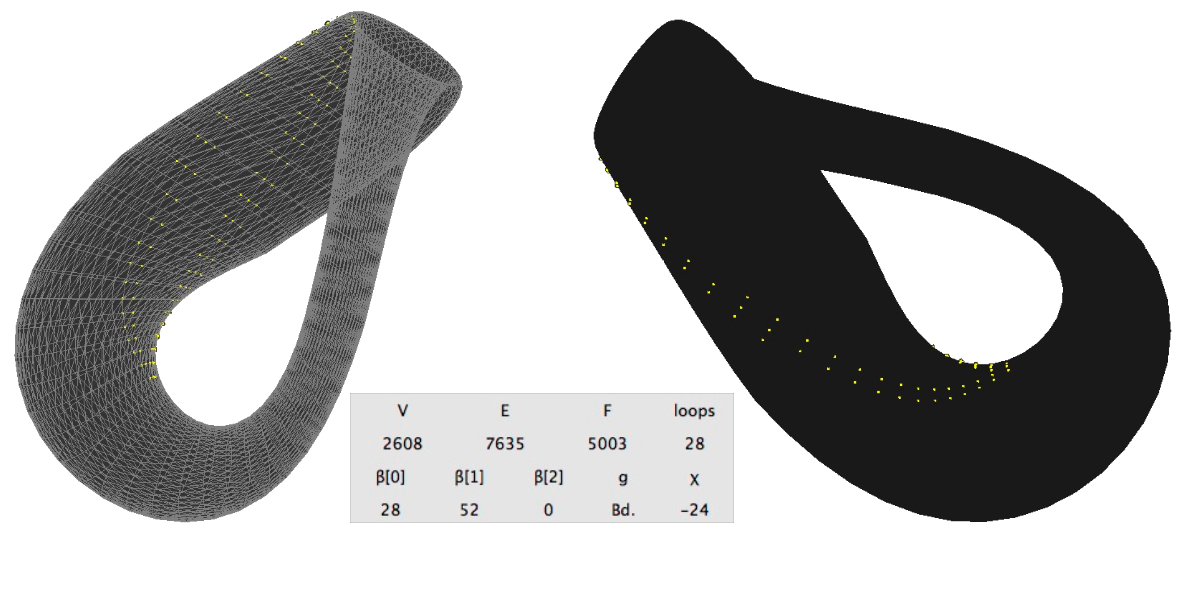
\includegraphics[width=0.70\textwidth]{klein_bottle.jpg}
\caption{The Klein bottle withstands filtration and decimation by our methods.}
\label{fig:klein_bottle}
\end{figure}


\section{Drawing on Meshes}
\label{topstoc3}

We now turn to the very heart and epitome of user-guidance, that is the explicit control over the decimation process\footnote{ User-guidance, somewhat unexpectedly, hasn't been of much interest in the last years as far as research papers are concerned. The work that still gets published, mostly reprises unimaginative adaptations of known decimation schemes to work with user input \citep[cf.][]{Ho2006}. This is astounding as the very first work already set a different trajectory by discussing among other things response times, i.e. work-flows \citep[cf.][]{Cignoni1998a}.}.\\
Although a major aspect of our work and an extremely powerful tool to selectively increase the fidelity of a mesh, the concept and implementation with ``TopStoc'' is strikingly unproblematic.
This is due to the fact that other decimation techniques are based on intangible error-bounds or priority queues, whereas our approaches rests on stochastics which is intuitively clear.
This way, instead of just attributing certain regions of a mesh with immunity to decimation, or fiddling with abstract rules and weights, the user just can literally sketching probability onto the base mesh.
%Bild
\begin{figure}[ht]
\centering
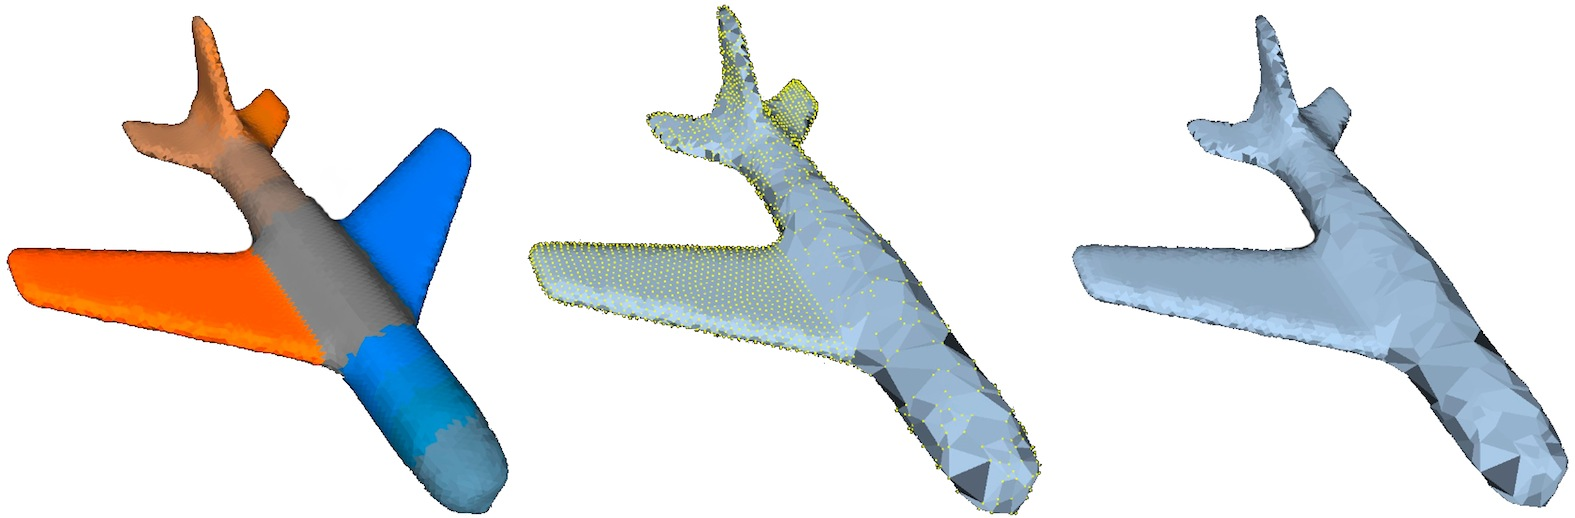
\includegraphics[width=1.0\textwidth]{planes.jpg}
\caption{Vertices on the wings of the plane are either kept or dismissed entirely (bright orange or dark blue). The body gradually gains geometric detail form top to back. On the plane in the middle, the then sampled vertices are shown and on the right is the final mesh alone.}
\label{fig:planes}
\end{figure}
In the example of figure \ref{fig:planes} the various parts of the plane model were painted with different probability levels.
Orange depicts values of relatively higher probability and blue levels of lower probability in respect to grey, which always conforms to the global target size that was set by the user.
Having the same effect as if each part of the model was processed individually with its own decimation ratio.\\  
This means that, for example, if the user adjusts the slider to a 0.5 the orange parts cover decimation ratios between $[0.5,1.0]$ and the likewise the blue areas cover $[0.5,0.0]$.
This seems to be problematic if the overall decimation ratio closes in on either boundary $1.0$ or $0.0$ and the colors encode less and less equal parts of the entire decimation range.
However the design was a deliberate decision, since this way one has a unambiguous and obvious feedback which parts were tweaked by the user to use less geometric detail and which parts needed to be boosted.
Furthermore the application offers the user a finely partitioning of each side, orange and blue, so that even in the most extreme cases the adjustability is ensured. 
%Bild
\begin{figure}[ht]
\centering
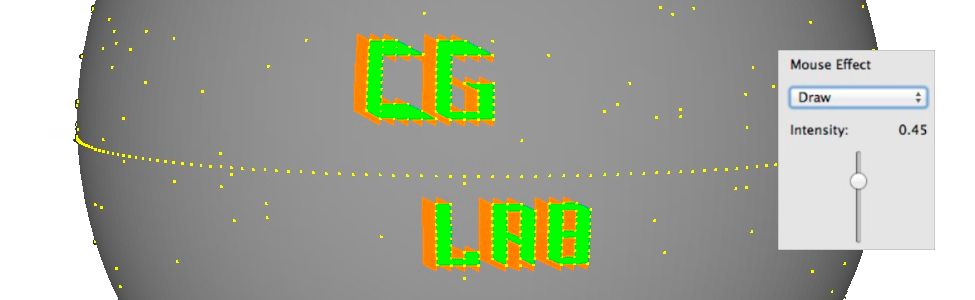
\includegraphics[width=0.80\textwidth]{controlpoints.jpg}
\caption{Besides the fuzzy painting of entire regions, the user has also the option to select a set of single elements and set their probability individualy.}
\label{fig:controlpoints}
\end{figure}\\
Note that the incorporation user-guidance does not impact the speed of the algorithm, as it only adds additional information for each vertex but does not require additional processing.
It is important to mention though, that once a region is painted with probability, the resulting mesh size after the decimation will deviate from the target size as user-input trumps it and an automatic adjustment enforcing the precise target size would lead to higher runtimes. 
%Bild
\begin{figure}[ht]
\centering
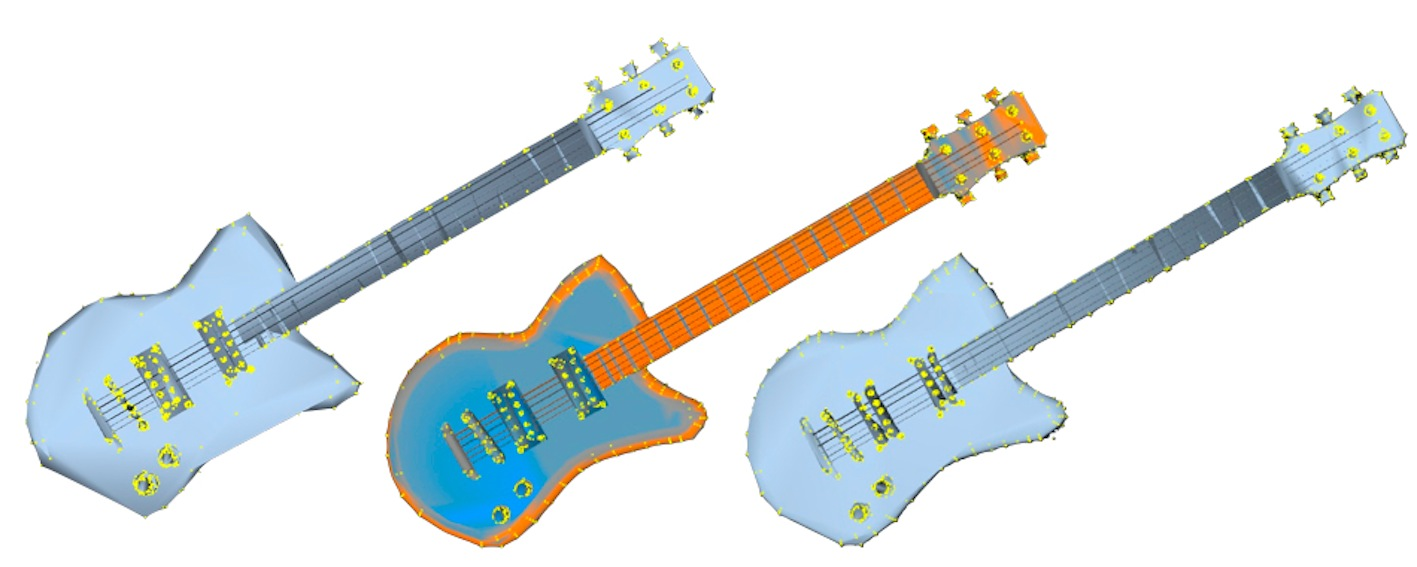
\includegraphics[width=1.00\textwidth]{sketchy_regions.jpg}
\caption{Another example of how user-assistance can lead to better results. Left is the unaltered result, right the improved version, note that both versions were sampled to the same vertex count $\pm$1\%.}
\label{fig:sketchy_regions}
\end{figure}

\newpage
\section{Back-face Subsampling \& Silhouette Preservation}
\label{topstoc41}

View-dependent decimation reckons that most of the time, only a fraction of the geometric detail is visible to us and that a good decimation scheme should exploit this.  
To leverage this fact, at least the direction of the camera is needed, achieving its full potential if a complete frustum is defined.
Together with the view-direction comes the concept of silhouettes, which are of pivotal importance for the perception of detail and geometric fidelity.
As early as 1996 appeared papers dealing with simplification methods that paid special attention to these details \citep[cf.][in which, not only view-dependencies but also decimation adapting to lighting conditions, gets discussed]{Xia1996}.
%Bild
\begin{figure}[ht]
\centering
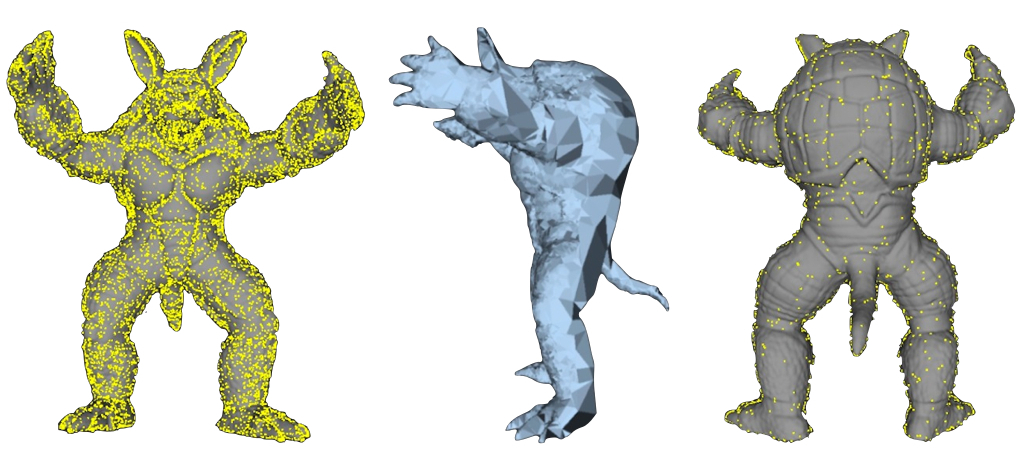
\includegraphics[width=1.0\textwidth]{armadillo_pov.jpg}
\caption{The \textit{Armadillo} model, showing the sampled vertices on the front and the back, with the resulting mesh in the middle.}
\label{fig:armadillo_pov}
\end{figure}\\
As in the case with user set decimation ratios, does the ``TopStoc'' algorithm lend itself almost effortless to an adaption for silhouette preservation and back-face culling.
Remember that the weight for vertices, as introduced in equation \ref{eq:vertex_weight} already uses normals.
Therefore this technique more or less inevitably suggests itself to be adapted, as soon as a view-vector $\mathrm{v}_{cam}$ is defined: $\mathrm{x}_{view}(\mathrm{v}) \,=\, (\textbf{n}^{T}_{v}\textbf{v}_{cam})/2$\\
Of course it is possible to introduce $\mathrm{v}_{cam}$ directly to equation \ref{eq:vertex_weight}, not adding it as an extra value to each vertex like we propose.
This undeniably would lessen the computational impact, offering back-face subsampling and silhouette preservation at no additional cost.
However this also means that all given weights have to be recalculated every time $\mathrm{v}_{cam}$ changes, even if only a normal decimation is desired.\\
%Bild
\begin{floatingfigure}[r]{0.31\textwidth}
%\begin{figure}[ht]
\center
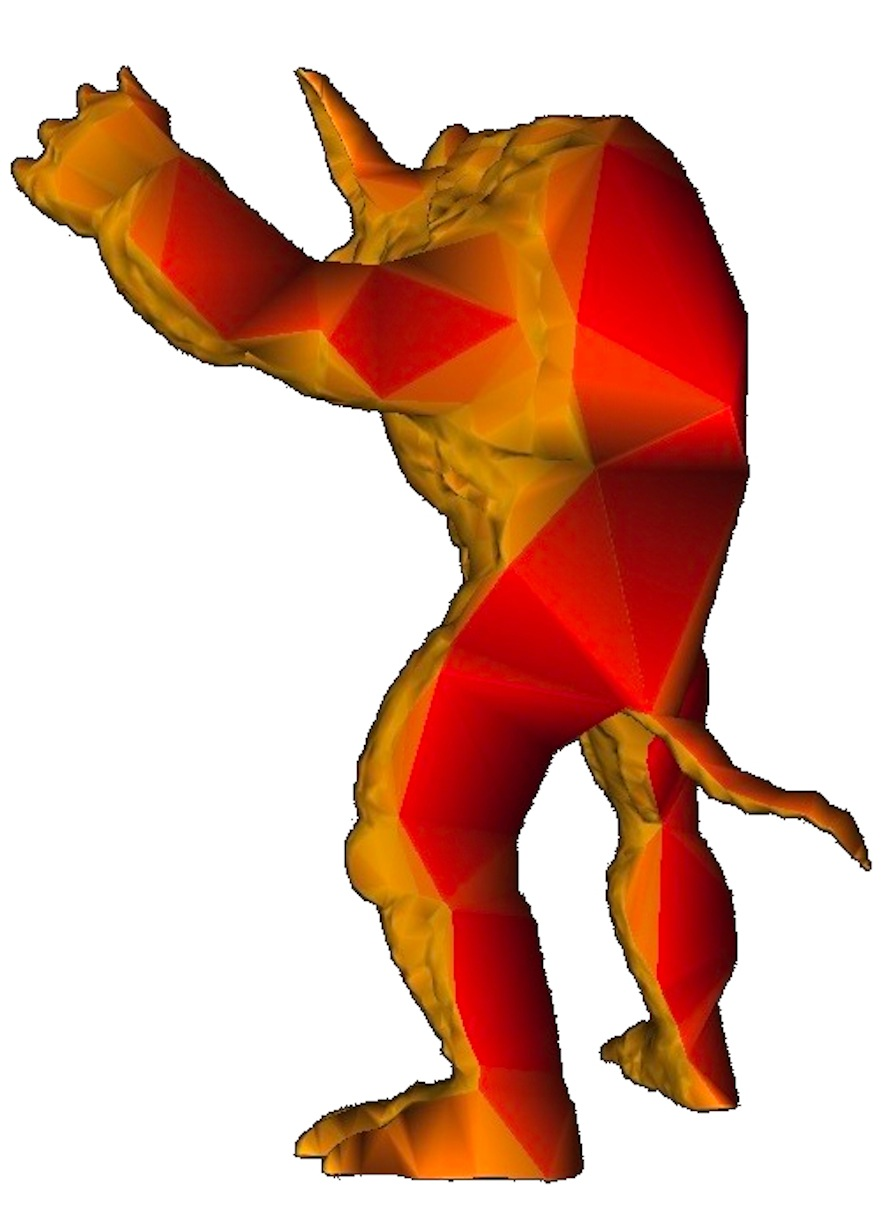
\includegraphics[width=0.29\textwidth]{armadillo_pov_hausdorff.jpg}
\caption{Errors per Triangle.}
\label{fig:armadillo_pov_hausdorff}
\end{floatingfigure}
%\end{figure}
In figure \ref{fig:armadillo_pov} the effect for a considerable lower sample rate on the back-face is shown.
Making use of a point of view aware decimation immediately drops the geometric complexity nearly by half, for the same accuracy of visible parts\footnote{ Depending on the geometry and the extend to which the object is concave -- with most organic models being very suitable, but hard surface models posing a bigger challenge.}.
To give a further impression of the results, we visualized the errors per triangle for the decimated mesh from figure \ref{fig:armadillo_pov}, see figure \ref{fig:armadillo_pov_hausdorff}.\\
Another interesting result is that since the ``TopStoc'' algorithm preserves the topology of an object we can cull faces on the backside of models altogether, still ending with a water-tight mesh at the end.
However, it is necessary to preserve vertices that lie on the silhouette to avoid artifacts that otherwise would result from the culling.\\
Silhouette preservation in itself is not an independent step as exactly the same normal calculation takes place.
The difference is that a values close to zero are dealt with more attention. 
Also for the practical applications it is necessary to define an interval for a graceful diminish, see the model on the right in figure \ref{fig:silhouette}.
This amends the problem that the area at the silhouette is not necessarily friendly towards such a treatment, unless the body is perfectly concave, obviously. 
%Bild
\begin{figure}[ht]
\centering
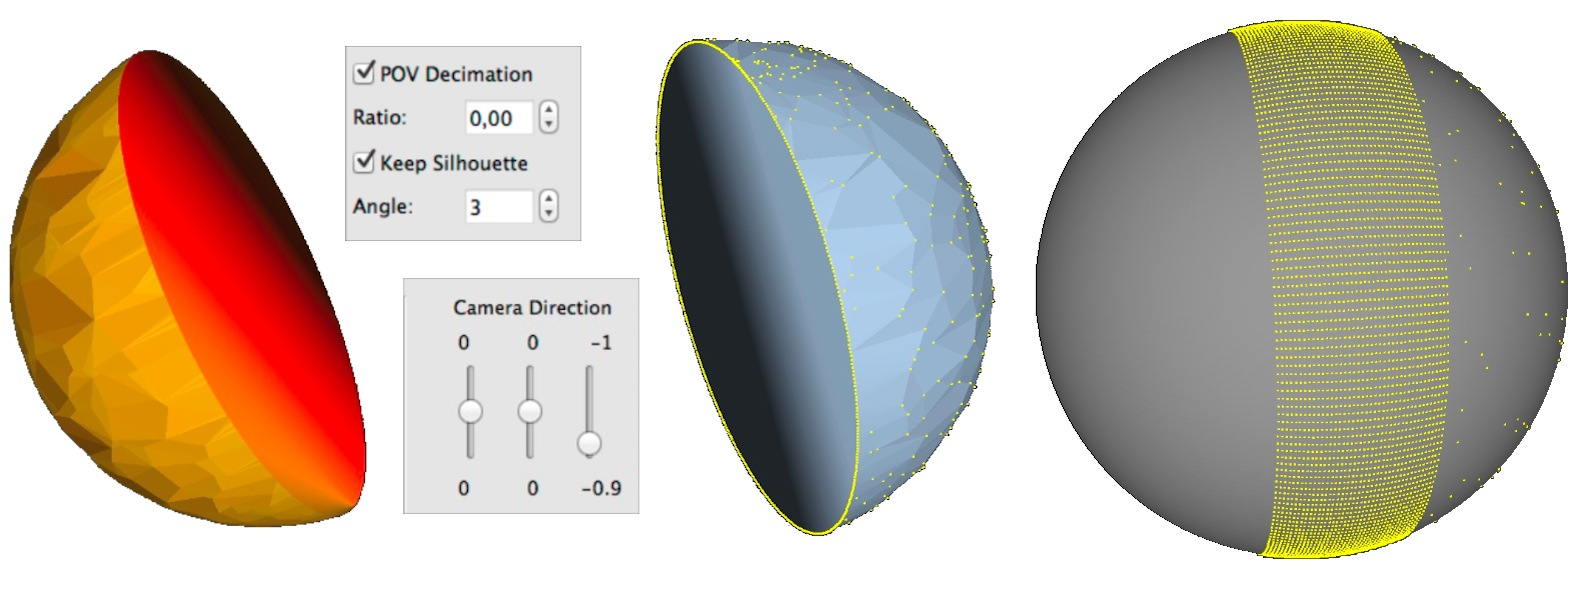
\includegraphics[width=1.0\textwidth]{silhouette.jpg}
\caption{Back-face culling and silhouette preservation are demonstrated on a sphere. On the left is the error visualization, next to it the GUI panel for the feature, in the middle is the decimated mesh with the sampled vertices colored and on right, the same model with a bigger aperture of the silhouette.}
\label{fig:silhouette}
\end{figure}
%Bild
\begin{figure}[ht]
\center
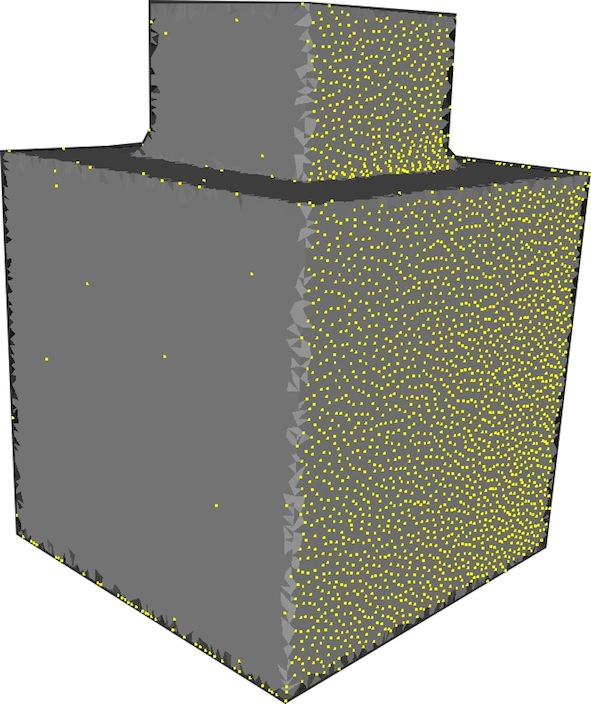
\includegraphics[width=0.29\textwidth]{pov_limitation.jpg}
\caption{Oversampling on ill-formed silhouette areas.}
\label{fig:pov_limitation}
\end{figure}\\
Unfortunately there are bad cases in which the preservation of the silhouettes not necessary fails, but yields really unwanted results.
Figure \ref{fig:pov_limitation} shows such a situation in which the silhouette coincides with a planar region, preserving way too many vertices.
This problem can be solved though by user intervention.
Painting with value -1, i.e. the dark blue, overrides any sampling decisions by the the algorithm.
All in all are the tools connected with the point of view a very helpful addition at negligible costs.


\section{Textures}
\label{topstoc42}

A key component in making any decimation method feasible for the actual adaptation in other field besides academia is the support for texture handling.
The role that textures play in fields like \textit{Computer Games} or the \textit{VFX} industry can not be overstated.
Actually the success of wrapping geometry with 2D images for various scenarios like bump-mapping, displacement information, dirt layers, etc. has to some extend fallen victim to its own success, but although more sophisticated solutions are available, like \texttt{Ptex}\footnote{ The idea behind this concept proposed by \textit{Burley} and \textit{Lacewell}, is to assigns an entirely separate texture per face, skipping the texture unwrap entirely.  The technique uses adjacency data to filter across faces, removing otherwise visible seams.}, conventional textures will be around for years to come \citep[cf.][\texttt{Ptex} opposed to MeshColors is a fully-fledged concept that has been already successfully used]{Burley2008}.\\
Because of this, it was important for us to include texture handling and support.
The problem when decimating meshes that normally hold textures is that highly visible artifacts appear if the boarders of the so called UV patches are not respected.

%Bild
\begin{figure}[htb]
\center
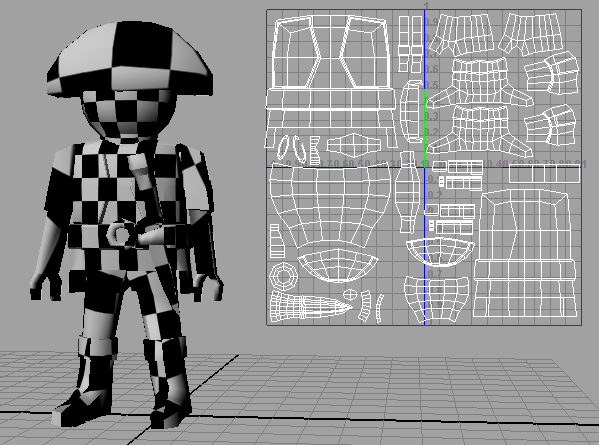
\includegraphics[width=0.66\textwidth]{uv_mapping.jpg}
\caption{Model with UV layout, image courtesy of \href{http://blogs.gscept.com/2008/sg2/index.php/page/2/index.html}{World Of RaftCraft}.}
\label{fig:uv_mapping}
\end{figure}\\
Figure \ref{fig:uv_mapping} shows a model together with its UV layout.
Note that color between the patches is normally black, so what one will typically see if a UV boarder vertex gets deleted is that the model has strange dark patches on its surface.\\
The easiest remedy to tackle this problem is to check which vertices have multiple texture coordinates as this defines the vertices on the boarder of UV patches.
Any of these can subsequently set to ``untouchable'' to ensure that no border gets lost.
This is what we implemented and is shown in figure \ref{fig:dec_texture}.
%Bild
\begin{figure}[htb]
\center
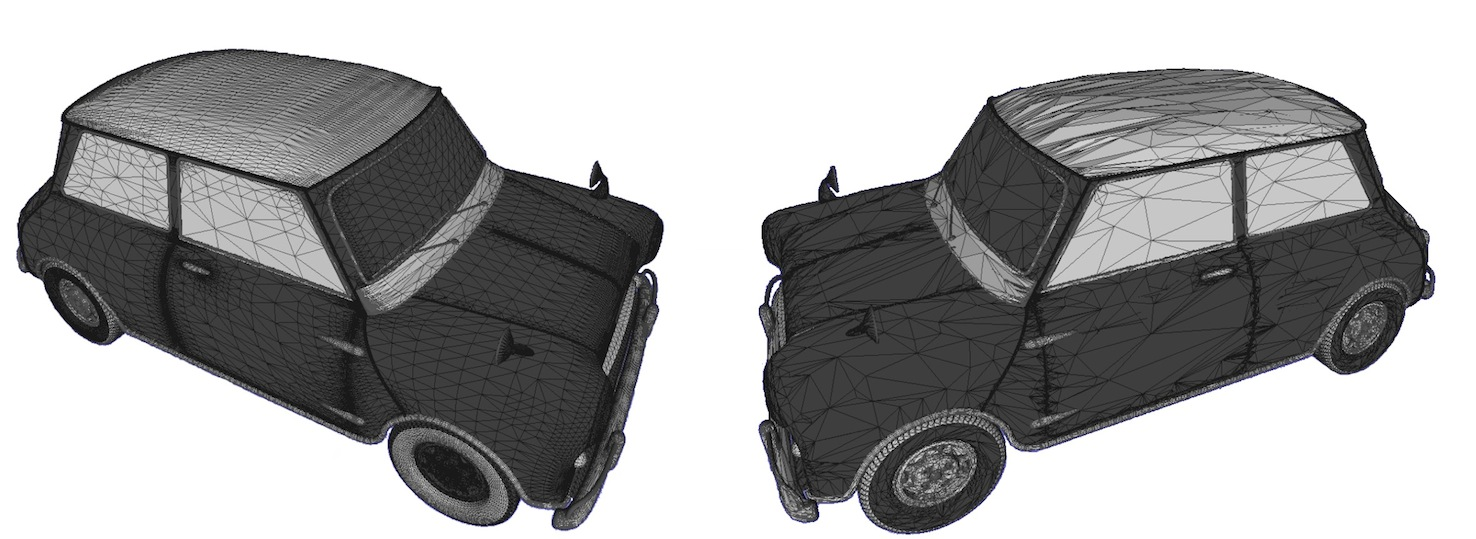
\includegraphics[width=1.0\textwidth]{dec_texture.jpg}
\caption{Modell ``Mini Cooper'' courtesy of \href{http://www.oyonale.com}{Oyonale}.}
\label{fig:dec_texture}
\end{figure}\\
The Mini on the left is the base mesh, on the right is the decimated version, note the high vertex density around the doors where a UV boarder resides.
At more sophisticated approach is to flood-fill the vertices of each patch to know, not only if a vertex lies on the boundary but also which specific patch it belong to.
This in turn makes it possible to redraw the texture and avoid artifacts altogether, well besides artifacts of distortion which would require even more subtle handling\footnote{ At this moment our reference implementation supports the preservation of vertices that have multiple texture coordinates, but we haven't pursuit any further so far.}. 


\section{Bounding Boxes \& Materials}
\label{topstoc43}

Last but not least is the support for bounding boxes and materials definitions.
These two items are not orthogonal to the rest of the tool set, so to say.
They \textit{only} facilitate the work for the user when dealing with models, but the effects could also be achieved if only using the previously described methods.

Support for bounding boxes entails the option to specify a series of cuboids.
Vertices that happen to be in any of such a volume get assigned one common weight.
This for instance is helpful to define frustums that cull an object.\\
Considering materials has a similar effect only that the familiarities of vertices are not defined by proximity but instead by the material definition given in the source file.
Almost all standards for geometry representation include such material definition and are normally used for rendering and shader binding.


\newpage
\section{Meassurements}
\label{topstoc5}

The evaluation of the results falls into two domains, on the one hand there is the individual perception of the user and on the other hand there are precise mathematical error bounds.
The user will typically make the final decision whether a certain asset holds up to his or her standards judging by the optical impression.
Yet, it is is also important to be able to get unequivocal data to rely on, for instance if simulations are involved.\\
We want to cater both scenarios as they are equally important.
Consequently we implemented one distinct tool for each one of them, not only to give feedback, but also to help guiding an iterative workflow.
% Bild
\vspace{0.2cm}
\begin{figure}[ht]
\begin{minipage}[b]{0.425\linewidth} \centering
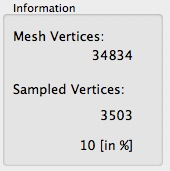
\includegraphics[height=3.0cm]{mesh_information.jpg}
\caption{Basic information, vertex count of the meshes.}
\label{fig:mesh_information}
\end{minipage}
\hspace{1.0cm}
\begin{minipage}[b]{0.5\linewidth}
\centering
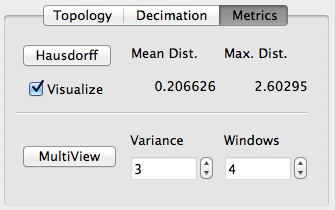
\includegraphics[height=3.0cm]{metrics_tab.jpg}
\caption{Metrics tab with the 'Hausdorff' and 'Multiview' section.}
\label{fig:metrics_tab}
\end{minipage}
\end{figure}\\
The basic information of the amount of vertices in the base mesh and the decimated mesh, is of course always shown.
Additionally, the tab labeled 'Metrics' offers the calculation and visualization of the Hausdorff distance, as well as the 'Multiview' tool which spawns new instances of the current decimation settings with limited variation, which will be both described in sections \ref{topstoc51} and \ref{topstoc52}.\\
Another useful utensil in assessing the decimation quality, is the turntable button.
When pressed, the mesh is placed in the center of the screen and the camera then gyrates two times around the model in an upwards spiral to show all the mesh from all direction.
%Bild
\begin{figure}[ht]
\centering
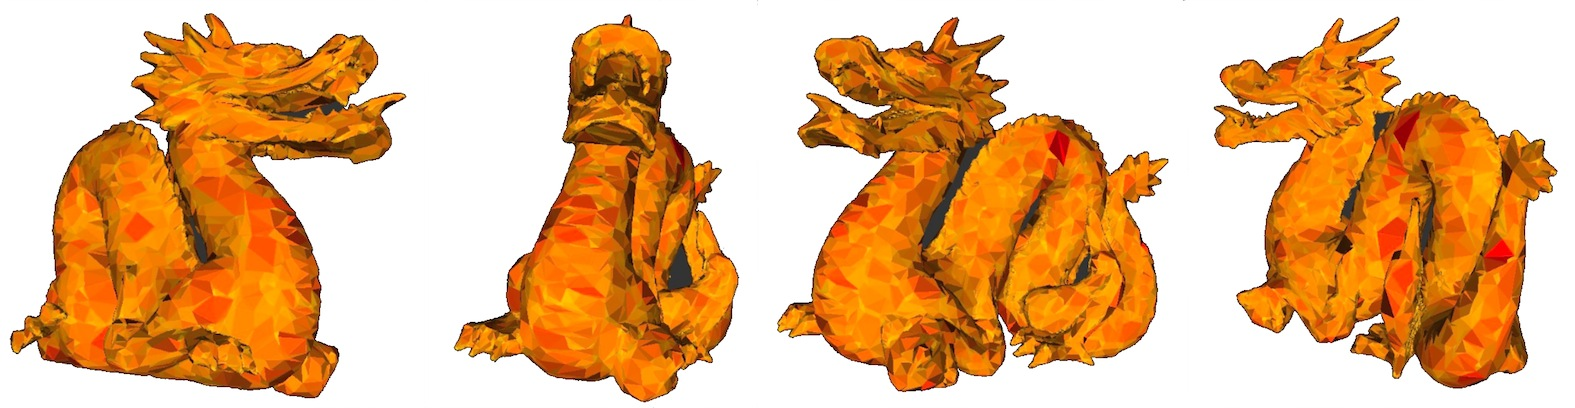
\includegraphics[width=0.85\textwidth]{turntable_dragon.jpg}
\caption{Turntable of the decimated dragon mesh, with Hausdorff distance visualized.}
\label{fig:turntable_dragon}
\end{figure}

\subsection{Hausdorff Distance}
\label{topstoc51}

In the case of 1D-signals and images, many distortion measurements have been studied.
They range from simple analytic methods such as the mean square error to very elaborate techniques based on the characteristics of human perception \citep[cf.][]{Winkler2001}.
Despite the constantly growing usage of 3D models, the distortion measurements for such data seem to be less thorough.
Still the predominant approach to compare two meshes is the \textit{Hausdorff distance}\footnote{ First introduced in the book \textit{Grundzüge der Mengenlehre}, published in 1914 and named after the German mathematician \textit{Felix Hausdorff} (1868 – 1942), one of the founders of modern topology. Technically the Hausdorff distance it is not a real distance function since it lacks symmetry. It is better to think of it in terms of set containment, for more information and examples see Appendix \ref{appendix5}.}, defined as:
\begin{equation} \label{eq:hausdorff}
\hspace*{0.5cm} d_{\mathrm H}(\mathcal{M},\mathcal{M}') = \sup_{p \in \mathcal{M}} \inf_{p' \in \mathcal{M}'} d(p, p')
\end{equation}
respectively the symmetric version:
\begin{equation}
d_{\mathrm H_{sym}}(\mathcal{M},\mathcal{M}') = \max \{\sup_{p \in \mathcal{M}} \inf_{p' \in \mathcal{M}'} d(p, p')~, \sup_{p' \in \mathcal{M}'} \inf_{p \in \mathcal{M}} d(p', p)\}
\end{equation}
Where the distance $d(p, p')$ between two points $p$ and $p'$ on the surfaces of the mesh $\mathcal{M}$ and it's simplified version $\mathcal{M}'$ is defined as: $d(p, p') = || p-p' ||$ with $||.||$ denoting the usual Euclidean norm.
We will refer to $d_{\mathrm H}(\mathcal{M},\mathcal{M}')$ as the forward distance, and to $d_{\mathrm H}(\mathcal{M}',\mathcal{M})$ as the backward distance.\\
The distance between any point $p$ belonging to $\mathcal{M}$ and $\mathcal{M}'$ can be computed analytically, since it can be reduced to the minimum of the distances between p and all the triangles $\mathcal{F}_{\mathcal{M}'}$.
It is worth noting that $p$ might not be a vertex of the list $\mathcal{V}_{\mathcal{M}}$ but any point on the surface.
Hence, although straightforward, the algorithm becomes too complex if implemented naively\footnote{ In fact, for each sample point $p$ it would be necessary to calculate the distance to all triangles $\mathcal{F}_{\mathcal{M}'}$ in order to find the minimum.
This leads to a complexity $\mathcal{O}(|p| \cdot |\mathcal{F}_{\mathcal{M}'}|)$, where $|p|$ is the number of sample points taken on $\mathcal{M}$ and $|\mathcal{F}_{\mathcal{M}'}|$ is the number of triangles.}.
To achieve reasonable running times we followed the implementation strategy described in the paper \textit{``Mesh: Measuring errors between surfaces using the hausdorff distance''}, where a cell partitioning strategy is used to greatly reduces the number of point-triangle distance evaluations.
Each triangles is sampled via a regular grid according to a length criterion, thus avoiding uniform sampling \citep[for more details see][especially chapter 3]{Aspert2002}.

By pressing the 'Hausdorff' button the backward distance is calculated and the numerical values for mean and maximum distances are shown.
Since the algorithm maintains a 1-1 correspondence between the sampled points and the base mesh, calculating the forward distance would yield little information and is omitted to save time.
%Bild
\begin{floatingfigure}[r]{0.31\textwidth}
\center
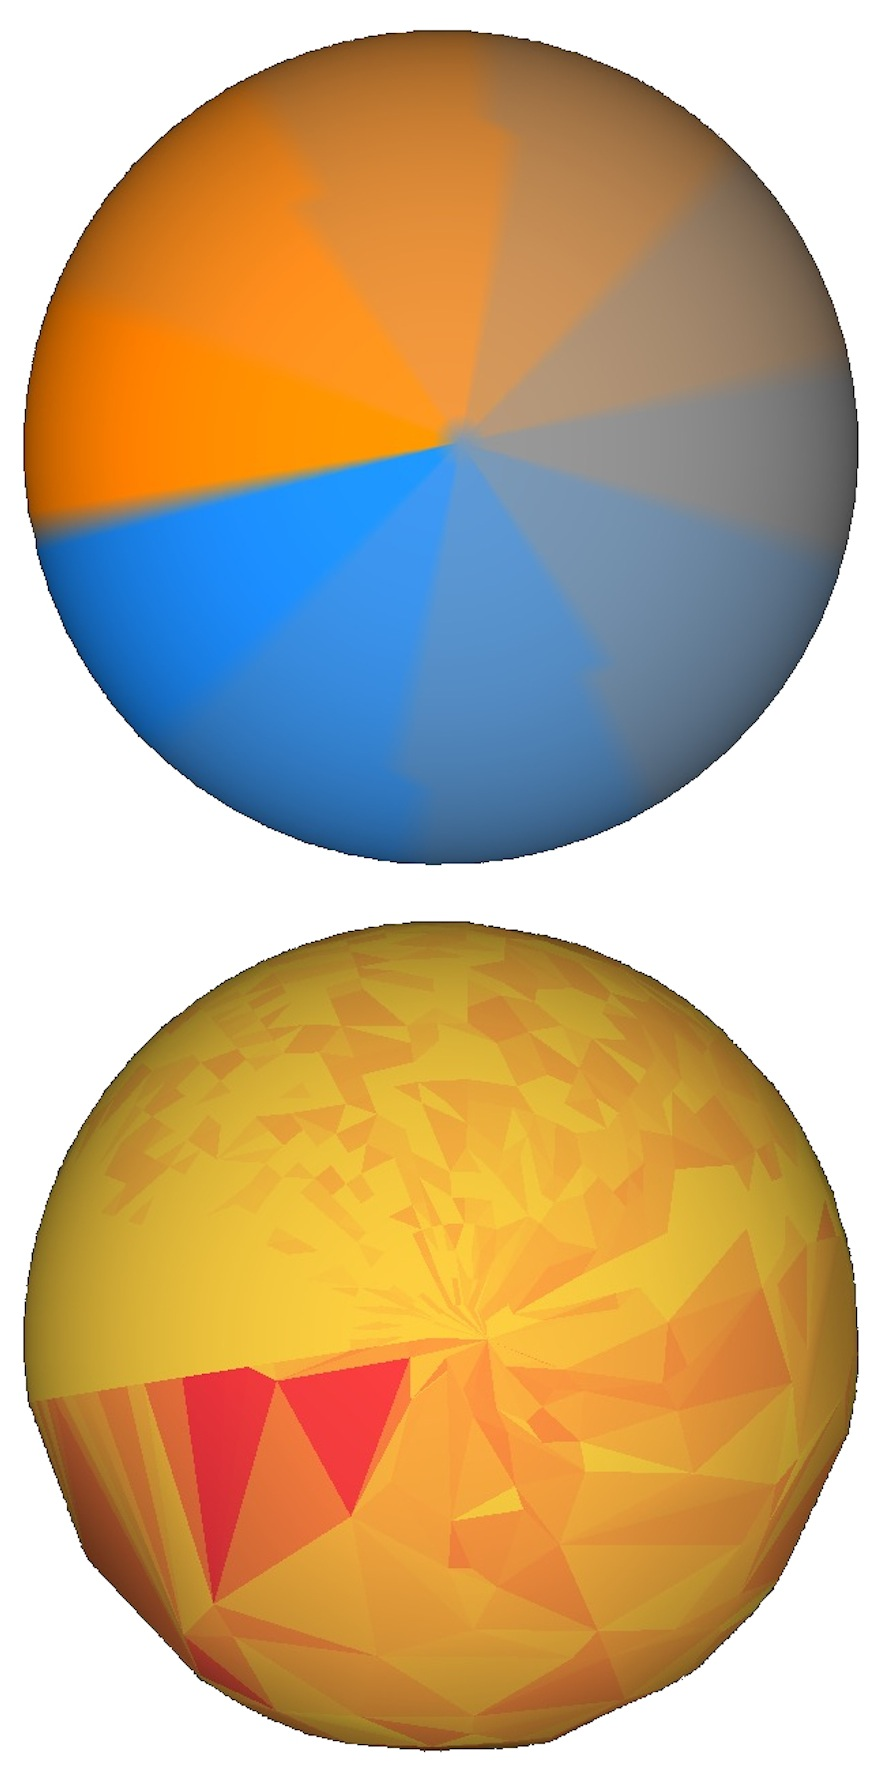
\includegraphics[width=0.29\textwidth]{hausdorff_colors.jpg}
\caption{Visualization Hausdorff.}
\label{fig:hausdorff_colors}
\end{floatingfigure}
More important for the practicality though, is that the normalized error values can be used to colorize the decimated mesh.
Thereby giving the user a clear representation of errors in the form of darkened triangles.
In image \ref{fig:hausdorff_colors} the upper sphere shows the gradually loosening of fidelity on the base mesh in colors.
Starting at the orange section on the upper left, where almost all vertices are sampled, the sampling rate steadily diminishes until it is below 1\% in the dark blue area.
The second lower sphere shows the decimated mesh with the visualization of the Hausdorff distance at each triangle.

The user can then switch between the the two visualization modes and selectively set control points on the base mesh to improve the quality in certain regions that would be otherwise undersampled.
In figure \ref{fig:hausdorff_control_points} the mesh is sampled at the same decimation rate of about 9,000 vertices two times, only deviating at less than 1\% of the total number.
However, for the second sampling, a series of control points were inserted in the areas of the cheek, forehead and the throat.
Giving a better overall result for the mean error of the Hausdorff distance.
%Bild
\begin{figure}[ht]
\centering
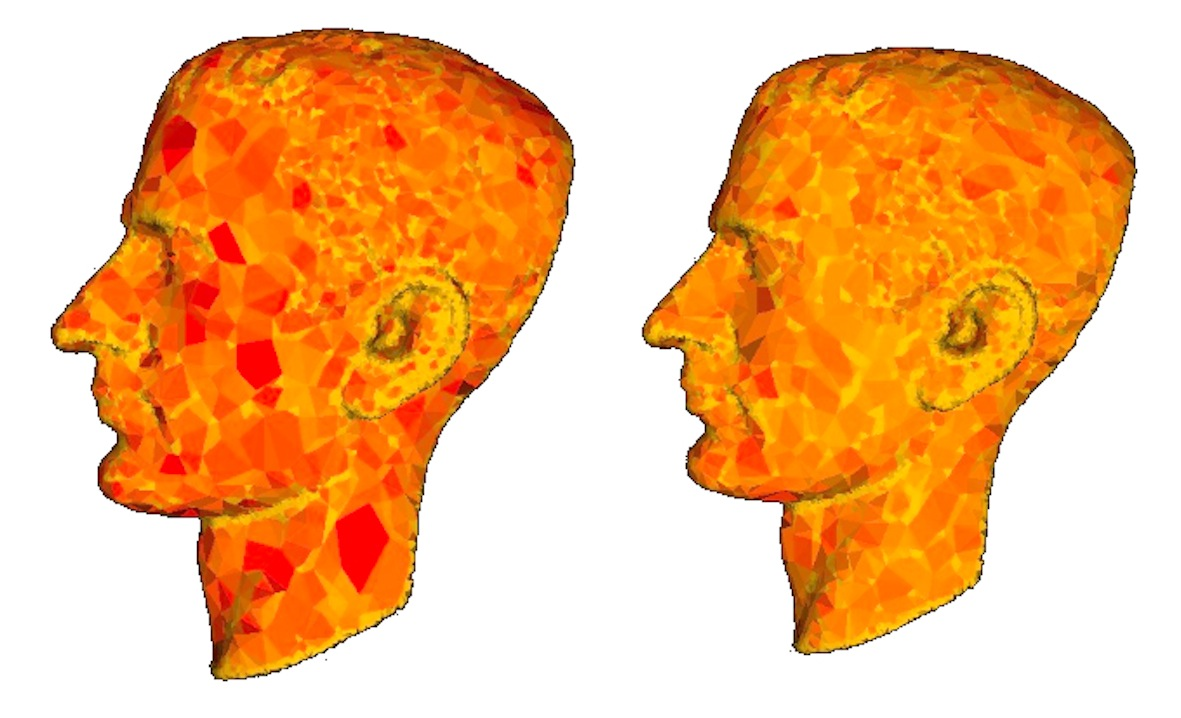
\includegraphics[width=0.55\textwidth]{hausdorff_control_points.jpg}
\caption{Two versions of a bust, with the same vertex count, but on the left hand side without control points to avoid undersampling.}
\label{fig:hausdorff_control_points}
\end{figure}

\subsection{Multiview}
\label{topstoc52}

With the Hausdorff distance at his disposal, the user is equipped to make very precise augmentations to a mesh and evaluate them quickly.
This complements the principle gauge tool for any decimation, that is the target size.
Even so, we think, that another tool has its place in this ensemble.\\
Multiview rests on the idea that it can be very beneficiary to get quick iterations with some variation of one and the same result.
The sampling algorithm is inherently stochastic and therefore will produce different versions albeit respecting constrains like user-set control points and the target size of the mesh.
We use this fact to offer the user the chance to create multiple instances of his decimation with just one single click.\\
%Bild
\begin{figure}[ht]
\centering
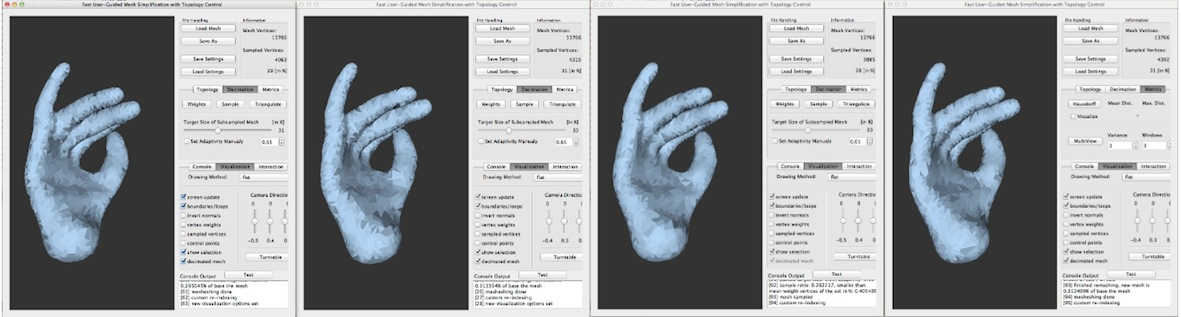
\includegraphics[width=1.0\textwidth]{multiview.jpg}
\caption{Four versions of a mesh with 3\% variance of the number of vertices.}
\label{fig:multiview}
\end{figure}\\
There are only two input variables that have to be defined, that is the maximal allowed variation in terms of \% mesh size and the number of instances that should be generated.
Using Multiview is possible because sampling and remeshing are comparatively inexpensive.
However with very large models it is advisable to restrict the newly instantiated windows to a small number.\\
Once the different models are created the user immediately sees whether it makes sense to persuit even lower decimation rates or if he already is at a threshold of accuracy he does not want to cross.
Besides giving fast visual feedback, Multiview can also be used to rapidly save multiple LOD versions if the variance is set to high percentages.
